\documentclass[11pt]{article}
\usepackage[a4paper,margin=28mm]{geometry}
\usepackage{amsmath,amssymb,amsthm,mathtools}
\usepackage[T1]{fontenc}
\usepackage{lmodern,microtype}
\usepackage{enumitem,booktabs,array}
\usepackage[font=small,labelfont=bf,margin=6mm]{caption}
\usepackage{tikz}
\usetikzlibrary{calc,arrows.meta,decorations.pathreplacing,decorations.pathmorphing,backgrounds,fit,shapes.geometric,positioning}
\usepackage[colorlinks=true,linkcolor=blue!55!black,urlcolor=blue!55!black,citecolor=green!35!black]{hyperref}
\usepackage[capitalise,nameinlink,noabbrev]{cleveref}

% ---------------------------------------------------------------------
% Theorem environments
% ---------------------------------------------------------------------
\newtheorem{theorem}{Theorem}[section]
\newtheorem{lemma}[theorem]{Lemma}
\newtheorem{proposition}[theorem]{Proposition}
\newtheorem{claim}{Claim}[theorem]
\theoremstyle{definition}
\newtheorem{definition}[theorem]{Definition}
\theoremstyle{remark}
\newtheorem{remark}[theorem]{Remark}
\crefname{claim}{Claim}{Claims}
\newtheorem{aclaim}{Claim}
\renewcommand{\theaclaim}{A.\arabic{aclaim}}
\crefname{aclaim}{Claim}{Claims}
\numberwithin{equation}{section}
\numberwithin{figure}{section}
\numberwithin{table}{section}

% ---------------------------------------------------------------------
% Macros
% ---------------------------------------------------------------------
\newcommand{\eps}{\varepsilon}
\newcommand{\E}{\mathbb{E}}
\renewcommand{\Pr}{\mathbb{P}}
\newcommand{\NN}{N}
\newcommand{\cP}{\mathcal{P}}
\newcommand{\cC}{\mathcal{C}}
\newcommand{\cT}{\mathcal{T}}
\newcommand{\cY}{\mathcal{Y}}
\newcommand{\cH}{\mathcal{H}}
\newcommand{\cL}{\mathcal{L}}
\newcommand{\cA}{\mathcal{A}}
\newcommand{\cM}{\mathcal{M}}
\newcommand{\cN}{\mathcal{N}}
\newcommand{\cB}{\mathcal{B}}
\newcommand{\cR}{\mathcal{R}}
\newcommand{\Hub}{\mathrm{Hub}}
\newcommand{\Fresh}{\mathrm{Fresh}}
\newcommand{\Lost}{\mathrm{Lost}}
\newcommand{\Def}{\mathrm{Def}}
\newcommand{\Used}{\mathrm{Used}}
\newcommand{\anc}{\mathrm{anc}}
\newcommand{\sh}{\mathrm{sh}}
\newcommand{\Rdon}{R^{\mathrm{don}}}
\newcommand{\Eas}{\mathbf{E}}
\newcommand{\paid}{\mathrm{paid}}
\newcommand{\oD}{o_D(n)}
\DeclareMathOperator{\lev}{lev}

% ---------------------------------------------------------------------
% Colours for figures (Okabe--Ito palette, safe for colour-blind readers)
% ---------------------------------------------------------------------
\definecolor{cHub}{HTML}{E69F00}
\definecolor{cPort}{HTML}{0072B2}
\definecolor{cFresh}{HTML}{009E73}
\definecolor{cRes}{HTML}{56B4E9}
\definecolor{cDel}{HTML}{D55E00}
\definecolor{cPool}{HTML}{CC79A7}
\tikzset{
  vtx/.style={circle,fill=black,inner sep=0pt,minimum size=4.2pt},
  hub/.style={circle,fill=cHub,draw=black!70,line width=.3pt,inner sep=0pt,minimum size=6pt},
  port/.style={circle,fill=cPort,draw=black!70,line width=.3pt,inner sep=0pt,minimum size=6pt},
  fresh/.style={circle,fill=cFresh,draw=black!70,line width=.3pt,inner sep=0pt,minimum size=6pt},
  pool/.style={rectangle,fill=cPool,draw=black!70,line width=.3pt,inner sep=0pt,minimum size=5.5pt},
  plain/.style={circle,fill=white,draw=black,line width=.5pt,inner sep=0pt,minimum size=5pt},
  edg/.style={line width=.9pt},
  res/.style={line width=1pt,cRes!80!black,dash pattern=on 3pt off 1.5pt},
  del/.style={line width=.8pt,cDel,dash pattern=on 2pt off 1.5pt},
  piece/.style={draw=black!75,line width=.6pt,fill=black!3},
  ancr/.style={draw=cRes!70!black,line width=.7pt,dashed,fill=cRes!10},
  lbl/.style={font=\small},
  box/.style={draw=black!70,line width=.5pt,rounded corners=2pt,fill=black!3,align=center,font=\footnotesize,inner sep=3pt},
  arr/.style={-{Stealth[length=2mm]},line width=.6pt,black!65},
}

\title{Decomposing a graph into linearly many cycles and edges}
\author{Claude Opus 5.5\\[2pt]
\small An AI-generated exposition of the proof claimed by Ryan Coffey~\cite{Cof}}
\date{1 October 2026}

\begin{document}
\maketitle

\begin{center}
\fbox{\parbox{0.9\textwidth}{\small\textbf{Status.} This write-up is entirely
AI-generated. At the time of posting (1~October 2026) no human has read or
understood this proof. It is meant as a stopgap: an intermediate artifact
between Coffey's proof claim and a final proof that humans have read, understood
and digested. It should not be cited as an established result.}}
\end{center}

\begin{abstract}
Erd\H{o}s and Gallai conjectured in the 1960s that the edge set of every graph
on $n$ vertices can be partitioned into $O(n)$ cycles and edges. Buci\'c and
Montgomery came within an iterated logarithm of this, proving the bound
$O(n\log^\star n)$: they peel off robust sublinear expanders in about
$\log^\star n$ rounds, and each round costs $O(n)$. We give a complete,
reorganised and simplified account of a proof of the full conjecture claimed by
Coffey. The new idea is that an expander found in one round is so much richer
than anything that happens two rounds later that it can serve as a reservoir of
connecting paths for all subsequent rounds. With these reservoirs each vertex
pays a constant only at its first two appearances. The few edges that still
cannot be closed into cycles are compressed into graphs with at most $n/4$
vertices in total, and these are decomposed by induction.
\end{abstract}

\tableofcontents

% =====================================================================
\section{Introduction}\label{sec:intro}
% =====================================================================

All graphs in this paper are finite and simple. For a graph $G$ let $f(G)$ be
the least number of cycles and single edges whose edge sets partition~$E(G)$.
In the 1960s Erd\H{o}s and Gallai conjectured that $f(G)=O(n)$ for every graph
$G$ on $n$ vertices; see~\cite{EGP} and Problem~\#184 of~\cite{Bloom}. The bound
would be best possible up to the constant: cycles contribute even degrees, so
in a graph in which every vertex has odd degree, every vertex is an end of a
single edge of the decomposition, and at least $n/2$ single edges are needed.

Repeatedly removing a longest cycle gives $f(G)=O(n\log n)$ (\cref{lem:egp}).
Lov\'asz~\cite{Lov} proved that every graph on $n$ vertices decomposes into at
most $n/2$ paths and cycles, and Pyber~\cite{Pyb} proved that the edges of
every such graph can be \emph{covered} by $n-1$ cycles and edges. For the
decomposition problem, Conlon, Fox and Sudakov~\cite{CFS} proved
$f(G)=O(n\log\log n)$, and Buci\'c and Montgomery~\cite{BM} proved
$f(G)=O(n\log^\star n)$, where $\log^\star$ is the iterated logarithm. This
paper presents a proof of the conjecture.

\begin{theorem}\label{thm:main}
There is an absolute constant $C$ such that $f(G)\le Cn$ for every graph $G$ on
$n$ vertices.
\end{theorem}

\paragraph{Provenance and status.} The argument below is a reorganisation and
simplification of a proof claimed by Coffey~\cite{Cof}, which in turn builds on
the method of Buci\'c and Montgomery~\cite{BM}. Coffey reports that his proof
was developed with substantial help from an AI system and that it comes with a
formalisation in Lean. That formalisation concerns his original manuscript and
not the version given here.

This write-up is entirely AI-generated. An earlier condensed draft was produced
by another AI system, and the present text was written by Claude Opus 5.5,
which also produced all figures and checked the argument, with the help of
independent AI reviews. At the time of posting, 1~October 2026, the proof has
not been read or understood by any human. It has not been refereed or formally
verified. Its purpose is to serve as a stopgap: an intermediate artifact
between Coffey's proof claim and a final proof that humans have read,
understood and digested. \Cref{sec:sources} lists the source of every
ingredient.

% ---------------------------------------------------------------------
\subsection{The strategy}\label{sec:strategy}
% ---------------------------------------------------------------------

This subsection explains the proof informally. Nothing in it is used later.

\paragraph{Rounds.} The method of Buci\'c and Montgomery~\cite{BM} runs in
rounds. A round starts from a graph $G_r\subseteq G$, on all $n$ vertices of
$G$, with average degree $d=d_r$; write $\lambda=\log d$. First one removes
cycles of length at least $d\lambda^2$, one at a time; there are at most
$n/(2\lambda^2)$ of them. The graph that remains has no long cycles, so all its
expanding subgraphs are small, since expanders contain long cycles. One then
splits it into robust sublinear expanders, called \emph{pieces}, of order at
most $d^2$, deleting a few edges along the way. The deleted edges, together
with the edges of a few small leftover parts, form the graph $G_{r+1}$ of the
next round, whose average degree is only polylogarithmic in~$d$. After about
$\log^\star n$ rounds the remaining graph has bounded average degree, and its
edges are simply taken as single edges.

In~\cite{BM} the edges inside the pieces of each round are decomposed using the
connectivity of expanders, at a cost proportional to the total order of the
pieces, which is $\Theta(n)$ per round. This is where the factor $\log^\star n$
comes from: a vertex can lie in pieces of every round, and it is paid for every
time.

\paragraph{Anchors.} The key observation, due to Coffey~\cite{Cof}, is that
earlier pieces are vastly richer than anything that happens two rounds later.
A piece of round $r$ is an $s_r$-expander with $s_r\approx\lambda_r^{50}$, so
all its degrees exceed $\lambda_r^{50}$. A piece of round $\ell\ge r+2$ has at
most $M_\ell\approx d_\ell^2$ vertices, and two rounds of polylogarithmic decay
give $M_\ell\le(\log\lambda_r)^{O(1)}$ (\cref{lem:scales}). So a piece of round
$r$ can set aside, for each later round, a random slice of its edges which is
still a robust expander with degrees far larger than anything in that round.
One round back is not enough, because a piece of round $r+1$ may have up to
$\lambda_r^{110}$ vertices.

Fix a round $\ell$. A vertex of a piece of round $\ell$ plays one of three roles
(\cref{fig:roles}):
\begin{itemize}[leftmargin=2em,itemsep=2pt]
\item a \emph{hub} lies in at least two pieces of round $\ell$. Hubs are rare:
summed over all rounds, the number of incidences between hubs and pieces is
$o(n)$;
\item a \emph{port} lies in exactly one piece of round $\ell$, and also lies in
a piece of some round $r\le\ell-2$, which we fix and call its \emph{anchor};
\item a \emph{fresh} vertex lies in exactly one piece of round $\ell$ and has no
anchor. Two rounds after a vertex first appears in a piece, it has an anchor,
so every vertex is fresh in at most two rounds.
\end{itemize}
Hubs and fresh vertices are dealt with inside their own piece at a cost of
$O(1)$ each, which is $O(n)$ in total. The main work is to deal with ports at a
total cost of $o(n)$ over all rounds.

\begin{figure}[t]
\centering
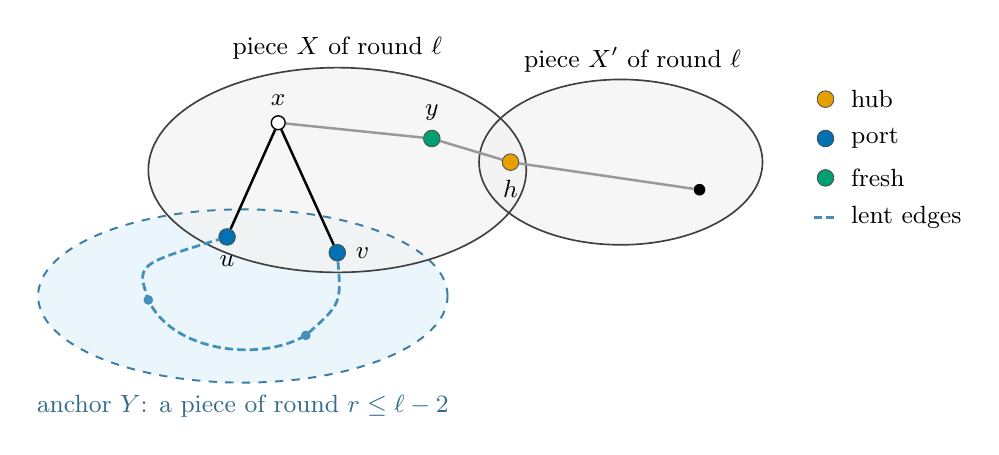
\begin{tikzpicture}[scale=1]
  \fill[cRes!12] (0,-1.0) ellipse (2.6 and 1.1);
  \fill[black!5,fill opacity=.7] (1.2,0.6) ellipse (2.4 and 1.3);
  \fill[black!5,fill opacity=.7] (4.8,0.7) ellipse (1.8 and 1.05);
  \draw[ancr,fill=none] (0,-1.0) ellipse (2.6 and 1.1);
  \draw[piece,fill=none] (1.2,0.6) ellipse (2.4 and 1.3);
  \draw[piece,fill=none] (4.8,0.7) ellipse (1.8 and 1.05);
  \node[lbl] at (1.2,2.15) {piece $X$ of round $\ell$};
  \node[lbl] at (4.95,2.0) {piece $X'$ of round $\ell$};
  \node[lbl,cRes!60!black] at (0,-2.4) {anchor $Y$: a piece of round $r\le\ell-2$};
  % vertices
  \node[port,label={[lbl]below:$u$}] (u) at (-0.2,-0.25) {};
  \node[port,label={[lbl]right:$v$}] (v) at (1.2,-0.45) {};
  \node[plain,label={[lbl]above:$x$}] (x) at (0.45,1.2) {};
  \node[fresh,label={[lbl]above:$y$}] (f) at (2.4,1.0) {};
  \node[hub,label={[lbl]below:$h$}] (h) at (3.4,0.7) {};
  \node[vtx] (z) at (5.8,0.35) {};
  % edges of round ell
  \draw[edg,black!40] (x)--(f)--(h)--(z);
  \draw[edg] (u)--(x)--(v);
  % lent path closing the cherry
  \draw[res] (v) .. controls (1.25,-1.1) .. (0.8,-1.5) .. controls (0.2,-1.85) and (-0.9,-1.7) .. (-1.2,-1.05) .. controls (-1.35,-0.6) .. (u);
  \node[vtx,cRes!80!black,minimum size=3.5pt] at (0.8,-1.5) {};
  \node[vtx,cRes!80!black,minimum size=3.5pt] at (-1.2,-1.05) {};
  % legend
  \begin{scope}[shift={(7.4,0.9)}]
    \node[hub] at (0,0.6) {}; \node[lbl,anchor=west] at (0.2,0.6) {hub};
    \node[port] at (0,0.1) {}; \node[lbl,anchor=west] at (0.2,0.1) {port};
    \node[fresh] at (0,-0.4) {}; \node[lbl,anchor=west] at (0.2,-0.4) {fresh};
    \draw[res] (-0.15,-0.9)--(0.15,-0.9); \node[lbl,anchor=west] at (0.2,-0.9) {lent edges};
  \end{scope}
\end{tikzpicture}
\caption{Roles of vertices in round $\ell$. The hub $h$ lies in two pieces of
round $\ell$. The ports $u,v$ lie only in $X$, and both have the old piece $Y$ as
their anchor. The edges $xu,xv$ of round $\ell$ leave $Y$, and together they form
a cherry $u\,x\,v$ with both ends in $Y$. A path of edges lent by $Y$ (dashed)
closes the cherry into a cycle. The vertex $y$ is fresh.}
\label{fig:roles}
\end{figure}

\paragraph{Cherries.} An edge of round $\ell$ never has both ends in an earlier
piece, because such edges were assigned to that piece when it was formed. So if
$u$ is a port with anchor $Y$, every edge $ux$ of round $\ell$ leaves $Y$. Fix
$Y$ and a vertex $x\notin Y$, and pair up the edges from $x$ to ports anchored at
$Y$. This gives \emph{cherries} $u\,x\,v$ with both ends in $Y$. The edges lent
by $Y$ can join the last vertex of one cherry to the first vertex of the next,
and so chain many vertex-disjoint cherries into a single long cycle
(\cref{fig:cherries}). In this way almost all edges at ports turn into few
cycles. What remains is at most one edge between each non-port $x$ and the
ports of each anchor.

\paragraph{The quotient.} A typical leftover edge joins a hub $h$ to a port $u$
with anchor $Y$. We extend it by a private edge $uw$ lent by $Y$ to a vertex $w$
of a sparse random \emph{pool}, and regard the path $h\,u\,w$ as a single edge
$hw$ of an auxiliary graph $Q_\ell$ whose vertices are hubs and pool vertices.
Leftover edges between two ports are treated in the same way, with a pool
vertex at each end. A cycle of $Q_\ell$ lifts to a cycle of $G$, and a single
edge of $Q_\ell$ lifts to at most two edges of $G$ (\cref{fig:quotient}).
Since hubs are rare and pools are sparse, the graphs $Q_\ell$ have at most $n/4$
vertices in total, so we can decompose them by induction on the number of
vertices.

\paragraph{Clearing.} Each piece is itself a robust expander, so it can absorb
all edges among any chosen set $P$ of its vertices into $O(|P|)$ cycles and
edges (\cref{lem:clear}). We use this for the hubs and fresh vertices, and for a
few ports that we sacrifice for technical reasons.

\paragraph{Building forwards, decomposing backwards.} All rounds are
constructed first. The decomposition then goes through the rounds in reverse
order (\cref{fig:timeline}). So when a piece $Y$ is finally decomposed, every
round that borrowed from $Y$ is finished. Only the edges that were actually
borrowed are removed from $Y$. All other edges of $Y$, including unused lent
edges, are decomposed together with its own edges.

\begin{figure}[t]
\centering
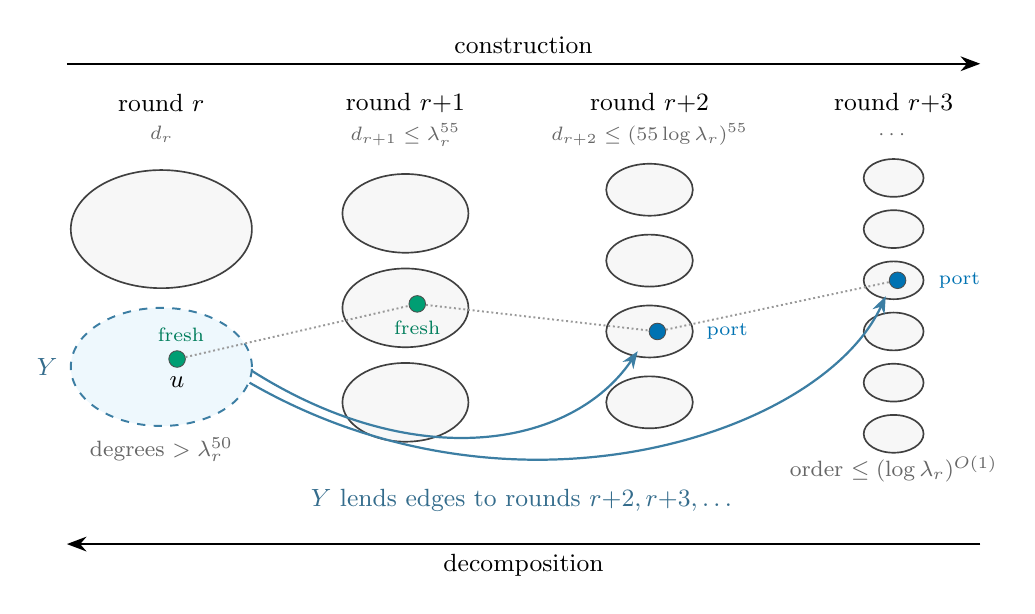
\begin{tikzpicture}[x=1cm,y=1cm]
  % column headers
  \foreach \x/\lab/\sub in {0/r/{d_r},3.1/r{+}1/{d_{r+1}\le\lambda_r^{55}},6.2/r{+}2/{d_{r+2}\le(55\log\lambda_r)^{55}},9.3/r{+}3/{\cdots}}{
    \node[lbl] at (\x,2.6) {round $\lab$};
    \node[font=\scriptsize,black!60] at (\x,2.2) {$\sub$};
  }
  % round r (large pieces)
  \draw[piece] (0,1.0) ellipse (1.15 and 0.75);
  \draw[ancr] (0,-0.75) ellipse (1.15 and 0.75);
  \node[lbl,cRes!60!black] at (-1.45,-0.75) {$Y$};
  % round r+1
  \draw[piece] (3.1,1.2) ellipse (0.8 and 0.5);
  \draw[piece] (3.1,0.0) ellipse (0.8 and 0.5);
  \draw[piece] (3.1,-1.2) ellipse (0.8 and 0.5);
  % round r+2
  \foreach \yy in {1.5,0.6,-0.3,-1.2}{\draw[piece] (6.2,\yy) ellipse (0.55 and 0.33);}
  % round r+3
  \foreach \yy in {1.65,1.0,0.35,-0.3,-0.95,-1.6}{\draw[piece] (9.3,\yy) ellipse (0.38 and 0.24);}
  % the vertex u
  \node[fresh] (u0) at (0.2,-0.65) {};
  \node[fresh] (u1) at (3.25,0.05) {};
  \node[port] (u2) at (6.3,-0.3) {};
  \node[port] (u3) at (9.35,0.35) {};
  \draw[black!40,densely dotted,line width=.7pt] (u0)--(u1)--(u2)--(u3);
  \node[lbl,anchor=north] at (0.2,-0.75) {$u$};
  \node[font=\scriptsize,cFresh!80!black,anchor=north] at (3.25,-0.04) {fresh};
  \node[font=\scriptsize,cFresh!80!black,anchor=south] at (0.25,-0.55) {fresh};
  \node[font=\scriptsize,cPort,anchor=west] at (6.8,-0.3) {port};
  \node[font=\scriptsize,cPort,anchor=west] at (9.75,0.35) {port};
  % lending arrows
  \draw[-{Stealth[length=2.2mm]},cRes!70!black,line width=.8pt] (1.15,-0.8) .. controls (3.2,-2.1) and (5.2,-1.8) .. (6.05,-0.55);
  \draw[-{Stealth[length=2.2mm]},cRes!70!black,line width=.8pt] (1.12,-0.95) .. controls (4.5,-2.9) and (8.4,-1.6) .. (9.2,0.15);
  \node[lbl,cRes!60!black] at (4.6,-2.45) {$Y$ lends edges to rounds $r{+}2,r{+}3,\dots$};
  % degree annotations
  \node[font=\footnotesize,black!60] at (0,-1.8) {degrees $>\lambda_r^{50}$};
  \node[font=\footnotesize,black!60] at (9.3,-2.05) {order $\le(\log\lambda_r)^{O(1)}$};
  % construction / decomposition arrows
  \draw[-{Stealth[length=2.5mm]},line width=.7pt] (-1.2,3.1) -- (10.4,3.1) node[midway,above,lbl] {construction};
  \draw[-{Stealth[length=2.5mm]},line width=.7pt] (10.4,-3.0) -- (-1.2,-3.0) node[midway,below,lbl] {decomposition};
\end{tikzpicture}
\caption{The rounds. Pieces get smaller from round to round, because the average
degree drops from $d$ to at most $(\log d)^{55}$. A vertex $u$ is fresh (green)
in the first two rounds in which it lies in a piece. After that it is a port
(blue) whose anchor $Y$ comes from at least two rounds earlier. Every piece
lends small random parts of its edges to all rounds at least two steps later.
The rounds are constructed from left to right and decomposed from right to left,
so every lender is decomposed after all of its borrowers.}
\label{fig:timeline}
\end{figure}

The argument thus reduces the problem to graphs with a quarter as many
vertices. The precise statement is as follows.

\begin{theorem}[Reduction]\label{thm:reduction}
There is an absolute constant $C_0$ such that for every graph $G$ on $n$
vertices there are graphs $Q_1,\dots,Q_k$ with
\[
\textstyle\sum_{i}|V(Q_i)|\le n/4
\qquad\text{and}\qquad
f(G)\le C_0n+2\sum_{i}f(Q_i).
\]
\end{theorem}

\begin{proof}[Proof of \cref{thm:main} from \cref{thm:reduction}]
We show $f(G)\le 2C_0n$ by induction on $n$. The case $n=0$ is trivial. For
$n\ge1$ each $Q_i$ has at most $n/4<n$ vertices, so by induction
$f(G)\le C_0n+2\sum_i2C_0|V(Q_i)|\le C_0n+C_0n$.
\end{proof}

% ---------------------------------------------------------------------
\subsection{Organisation}\label{sec:organisation}
% ---------------------------------------------------------------------

\Cref{fig:deps} shows how the results depend on each other. \Cref{sec:prelim}
fixes notation and collects the classical tools. \Cref{sec:hierarchy} builds
the rounds and proves their structural properties. \Cref{sec:linking} states
the linking lemma, which is behind every connection we make through an
expander; its proof, an adaptation of the method of~\cite{BM}, is in
\cref{app:linking}. \Cref{sec:three} proves three self-contained decomposition
lemmas: clearing a set of vertices, closing cherries, and building the
quotient. \Cref{sec:proof} puts everything together and proves
\cref{thm:reduction}. \Cref{sec:sources} lists the sources.

A reader who wants the main line of the argument can read \cref{sec:strategy},
the statements in \cref{sec:hierarchy,sec:linking}, \cref{sec:three} and
\cref{sec:proof}, and skip the proofs of \cref{sec:hierarchy} and the
appendix.

\begin{figure}[t]
\centering
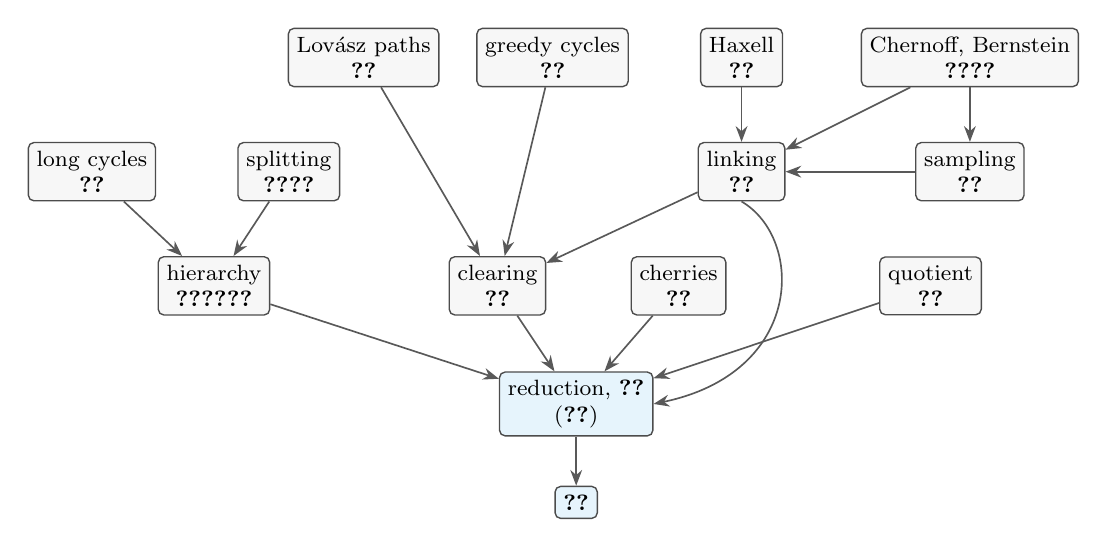
\begin{tikzpicture}
  % top row: classical tools
  \node[box] (lov) at (1.7,2.9) {Lov\'asz paths\\\cref{lem:lovasz}};
  \node[box] (egp) at (4.1,2.9) {greedy cycles\\\cref{lem:egp}};
  \node[box] (hax) at (6.5,2.9) {Haxell\\\cref{thm:haxell}};
  \node[box] (prob) at (9.4,2.9) {Chernoff, Bernstein\\\cref{lem:chernoff,lem:freedman}};
  % middle row
  \node[box] (long) at (-1.75,1.45) {long cycles\\\cref{lem:longcycle}};
  \node[box] (split) at (0.75,1.45) {splitting\\\cref{lem:split,lem:tree}};
  \node[box] (link) at (6.5,1.45) {linking\\\cref{lem:link}};
  \node[box] (samp) at (9.4,1.45) {sampling\\\cref{lem:sample}};
  % bottom row
  \node[box] (hier) at (-0.2,0) {hierarchy\\\cref{lem:hierarchy,lem:scales,lem:bookkeeping}};
  \node[box] (clear) at (3.4,0) {clearing\\\cref{lem:clear}};
  \node[box] (cher) at (5.7,0) {cherries\\\cref{lem:cherry}};
  \node[box] (quot) at (8.9,0) {quotient\\\cref{lem:quotient}};
  % conclusion
  \node[box,fill=cRes!15] (red) at (4.4,-1.5) {reduction, \cref{thm:reduction}\\(\cref{sec:proof})};
  \node[box,fill=cRes!15] (main) at (4.4,-2.75) {\cref{thm:main}};
  % arrows
  \draw[arr] (long) -- (hier);
  \draw[arr] (split) -- (hier);
  \draw[arr] (lov) -- (clear);
  \draw[arr] (egp) -- (clear);
  \draw[arr] (hax) -- (link);
  \draw[arr] (prob) -- (samp);
  \draw[arr] (prob) -- (link);
  \draw[arr] (samp) -- (link);
  \draw[arr] (link) -- (clear);
  \draw[arr] (hier) -- (red);
  \draw[arr] (clear) -- (red);
  \draw[arr] (cher) -- (red);
  \draw[arr] (quot) -- (red);
  \draw[arr] (link.south) .. controls (7.3,0.6) and (7.3,-1.1) .. (red.east);
  \draw[arr] (red) -- (main);
\end{tikzpicture}
\caption{How the results depend on each other. The three decomposition lemmas
of \cref{sec:three} are independent of the hierarchy; they meet only in the
assembly of \cref{sec:proof}, which also uses the linking lemma (and with it the
sampling lemma) to equip the pieces with reservoirs. The clearing lemma also uses
the sampling lemma directly.}
\label{fig:deps}
\end{figure}

% =====================================================================
\section{Preliminaries}\label{sec:prelim}
% =====================================================================

\subsection{Notation}
For a graph $H$ we write $|H|$ for its number of vertices and $e(H)$ for its
number of edges. For $U\subseteq V(H)$, $H[U]$ is the induced subgraph and
\[
\NN_H(U)=\{v\in V(H)\setminus U: v\text{ has a neighbour in }U\}
\]
is the \emph{external} neighbourhood of $U$. For disjoint $A,B\subseteq V(H)$,
$E_H(A,B)$ is the set of edges with one end in $A$ and the other in $B$. For a
set $F$ of edges, $H-F$ is obtained by deleting $F$ and keeping all vertices,
and $\deg_F(v)$ is the number of edges of $F$ at $v$. For a set $E$ of edges
and a set $P$ of vertices, $E[P]$ is the set of edges of $E$ with both ends
in~$P$. All logarithms are to base two; $\ln$ is the natural logarithm.

An \emph{object} is a cycle or a single edge, identified with its edge set. A
\emph{decomposition} of a set $F$ of edges is a partition of $F$ into objects,
and $f(F)$ is the least number of objects in a decomposition of $F$; for a graph
$H$, $f(H)=f(E(H))$. Clearly $f(F)\le|F|$, and $f(F\cup F')\le f(F)+f(F')$ for
disjoint $F,F'$. To \emph{pay for} an edge means to use it as a single-edge
object.

A path is \emph{through} a set $V$ if all its interior vertices lie in $V$.
Its ends are unrestricted, and a single edge is a path through every set.

\begin{definition}[Linking]\label{def:linking}
Let $H$ be a graph, $V\subseteq V(H)$ and $t\ge1$. We say that $H$ \emph{links
through $V$ with multiplicity $t$} if the following holds for every multiset
$\cP$ of pairs of distinct vertices of $H$ in which every vertex lies in at most
$t$ pairs, counted with multiplicity: there are pairwise edge-disjoint paths
$P_\pi$, $\pi\in\cP$, in $H$, such that $P_\pi$ joins the two vertices of $\pi$
and is through~$V$.
\end{definition}

This is the notion of path connectivity of~\cite[Definition~7]{BM}, without
the bound on the lengths of the paths, which we never need.

\subsection{Three classical facts}

\begin{lemma}[Paths; Lov\'asz~\cite{Lov}, see {\cite[Corollary~22]{BM}}]\label{lem:lovasz}
The edges of every graph can be decomposed into paths so that every vertex is
an end of at most two of the paths. In particular, if every edge of a graph has
both ends in a set $W$, then its edges decompose into at most $|W|$ paths.
\end{lemma}

The second statement follows from the first because every path has two
distinct ends.

\begin{lemma}[Greedy cycle removal]\label{lem:egp}
Every graph $H$ on $h\ge1$ vertices satisfies $f(H)\le h(\log h+1)$.
\end{lemma}

\begin{proof}
If a graph on $h$ vertices has $m>h$ edges, then it contains a cycle of length
greater than $m/h$. Indeed, delete vertices of degree less than $m/h$ one at a
time. Each deletion removes fewer than $m/h$ edges and at most $h$ vertices are
deleted, so fewer than $m$ edges are removed, and the process stops at a
nonempty subgraph of minimum degree at least $m/h>1$. All neighbours of the
first vertex $v_0$ of a longest path $v_0v_1\cdots v_k$ in this subgraph lie on
the path. If $v_i$ is the last of them, then $i\ge m/h$, and
$v_0v_1\cdots v_iv_0$ is a cycle of length $i+1>m/h$.

Now remove such cycles from $H$ while it has more than $h$ edges. While the
number $m$ of remaining edges lies in $(2^ih,2^{i+1}h]$, every removed cycle has
more than $2^i$ edges, so at most $h$ cycles are removed. As $m\le h^2/2$, only
the ranges with $2^i<h/2$ occur, and there are at most $\log h$ of them. So at
most $h\log h$ cycles are removed, and at most $h$ edges remain, which we pay
for.
\end{proof}

This is the classical bound $f(G)=O(n\log n)$, observed already by Erd\H{o}s
and Gallai; see~\cite{CFS,BM}.

\begin{theorem}[Haxell~\cite{Hax}]\label{thm:haxell}
Let $h\ge1$ and let $\cA_1,\dots,\cA_q$ be families of sets of size at most $h$.
Suppose that for every nonempty $I\subseteq[q]$ and every set $S$ with
$|S|\le(2h-1)(|I|-1)$, some member of some $\cA_i$ with $i\in I$ is disjoint
from $S$. Then there are pairwise disjoint sets $A_1\in\cA_1,\dots,A_q\in\cA_q$.
\end{theorem}

In Haxell's formulation, the families form a bipartite hypergraph in which each
edge consists of one index $i$ together with a member of $\cA_i$, so edges have
at most $r=h+1$ vertices, and the bound $(2r-3)(|I|-1)$ on transversals is the
bound above.

\subsection{Probability}

\begin{lemma}[Chernoff bounds; see~{\cite[Theorems~2.1 and~2.8]{JLR}}]\label{lem:chernoff}
Let $X$ be a sum of independent indicator variables and $0<\delta\le1$. If
$\E X\ge\mu$ then $\Pr(X\le(1-\delta)\mu)\le e^{-\delta^2\mu/2}$, and if
$\E X\le\mu$ then $\Pr(X\ge(1+\delta)\mu)\le e^{-\delta^2\mu/3}$.
\end{lemma}

We also need a Bernstein-type inequality for functions of independent bits.
It follows by applying Freedman's martingale inequality~\cite{Fre} to the
exposure martingale; see also~\cite{McD}.

\begin{lemma}[Bernstein inequality for bounded differences]\label{lem:freedman}
Let $\xi_1,\dots,\xi_k$ be independent $\{0,1\}$-valued random variables with
$\Pr(\xi_i=1)=p_i$, and let $Z=\phi(\xi_1,\dots,\xi_k)$, where changing $\xi_i$
alone changes $\phi$ by at most $c_i\le c$. Put
$\sigma^2=\sum_ip_i(1-p_i)c_i^2$. Then for all $x>0$,
\[
\Pr(Z\le\E Z-x)\le\exp\Bigl(-\frac{x^2}{2(\sigma^2+cx/3)}\Bigr).
\]
\end{lemma}

\begin{proof}
Let $Z_i=\E[Z\mid\xi_1,\dots,\xi_i]$. Given $\xi_1,\dots,\xi_{i-1}$, let
$g(y)=\E[Z\mid\xi_1,\dots,\xi_{i-1},\xi_i=y]$. By independence $g(1)-g(0)$ is
an average of differences of $\phi$, so $|g(1)-g(0)|\le c_i$. Hence the
martingale difference $Z_i-Z_{i-1}=g(\xi_i)-\E g(\xi_i)$ is bounded by $c$ in
absolute value and has conditional variance
$p_i(1-p_i)(g(1)-g(0))^2\le p_i(1-p_i)c_i^2$. Freedman's inequality~\cite{Fre},
applied to the martingale $-Z_i$, now gives the bound.
\end{proof}

\subsection{Robust sublinear expanders}

Throughout the paper we fix
\[
\eps=1/32.
\]

\begin{definition}[Expanders]\label{def:expander}
Let $s\ge0$. A graph $H$ on $N\ge2$ vertices is an \emph{$s$-expander} if
\[
|\NN_{H-F}(U)|\ge\frac{\eps|U|}{\log^2N}
\qquad\text{whenever } 1\le|U|\le\tfrac23N\text{ and }F\subseteq E(H),\ |F|\le s|U|.
\]
\end{definition}

Sublinear expanders were introduced by Koml\'os and
Szemer\'edi~\cite{KS1,KS2}. The robust form, in which up to $s|U|$ edges may be
deleted, was introduced independently by Haslegrave, Kim and Liu~\cite{HKL} and
by Sudakov and Tomon~\cite{ST}. In the notation of~\cite[Definition~11]{BM}, our
$s$-expanders are the $(\eps,s)$-expanders with $\eps=2^{-5}$. See~\cite{Let}
for a survey. We use two simple consequences of the definition.
\begin{itemize}[leftmargin=2em,itemsep=1pt]
\item An $s$-expander has minimum degree greater than $s$. Indeed, for a vertex
$v$, taking $U=\{v\}$ and $F$ the set of edges at $v$ gives
$\NN_{H-F}(U)=\varnothing$, so $|F|>s$. In particular $N>s+1$.
\item An $s$-expander is an $s'$-expander for every $s'\le s$.
\end{itemize}

% =====================================================================
\section{Expanders and the hierarchy of rounds}\label{sec:hierarchy}
% =====================================================================

This section builds the rounds. \Cref{sec:longcycles,sec:splitting} prove the
two facts about expanders that the rounds rest on: expanders contain long
cycles, and every graph splits into expanders that overlap little.
\Cref{sec:rounds} defines the rounds, and \cref{sec:roles} defines the roles
of vertices and proves that the quantities charged to them are summable.

\subsection{Long cycles}\label{sec:longcycles}

Buci\'c and Montgomery use a depth-first search to find a cycle of length
$\Omega(N/\log^4N)$ in a $0$-expander on $N$ vertices~\cite[Lemma~25]{BM}. A
slightly different use of depth-first search, a now standard tool for long paths
and cycles~\cite{Kri}, gives a better bound with less work.

\begin{lemma}[Long cycles in expanders]\label{lem:longcycle}
Every $0$-expander $H$ on $N\ge2^{20}$ vertices contains a cycle of length at
least $N/(2^8\log^2N)$.
\end{lemma}

\begin{proof}
$H$ is connected: otherwise a smallest component $K$ has $|K|\le N/2$ and
$\NN_H(K)=\varnothing$, which contradicts expansion. Let $T$ be a depth-first
search tree of $H$ with root $o$. Every edge of $H$ joins a vertex to one of
its ancestors in $T$. For a vertex $y$ let $T_y$ be the set of its descendants,
including $y$.

Put $k=\lfloor N/2\rfloor$, and let $v$ be a vertex of maximum depth with
$|T_v|>k$. The sets $T_c$, for the children $c$ of $v$, partition
$T_v\setminus\{v\}$. Each has size at most $k$, and together they have size at
least $k$. So we can choose a union $U$ of some of them with $k/2\le|U|\le k$:
take one $T_c$ of size at least $k/2$ if there is one, and otherwise add sets
$T_c$ one at a time until the size first reaches $k/2$.

Since $U$ is a union of whole subtrees hanging from $v$, every vertex outside
$U$ with a neighbour in $U$ is an ancestor of that neighbour, and hence lies on
the path from $o$ to $v$ in $T$ (\cref{fig:dfs}). Note that $v$ itself lies in
$\NN_H(U)$. As $|U|\le N/2$, expansion gives
\[
q:=|\NN_H(U)|\ge\frac{\eps k}{2\log^2N}\ge\frac{N}{2^8\log^2N}\ge 2.
\]
Let $x$ be the vertex of $\NN_H(U)$ closest to $o$, and let $u\in U$ be a
neighbour of $x$. As $q\ge2$, $x$ is a proper ancestor of $v$. So the path from
$x$ to $u$ in $T$ has length at least two, and it passes through all $q$
vertices of $\NN_H(U)$. Together with the edge $ux$ it forms a cycle of length
at least $q+1$.
\end{proof}

\begin{figure}[t]
\centering
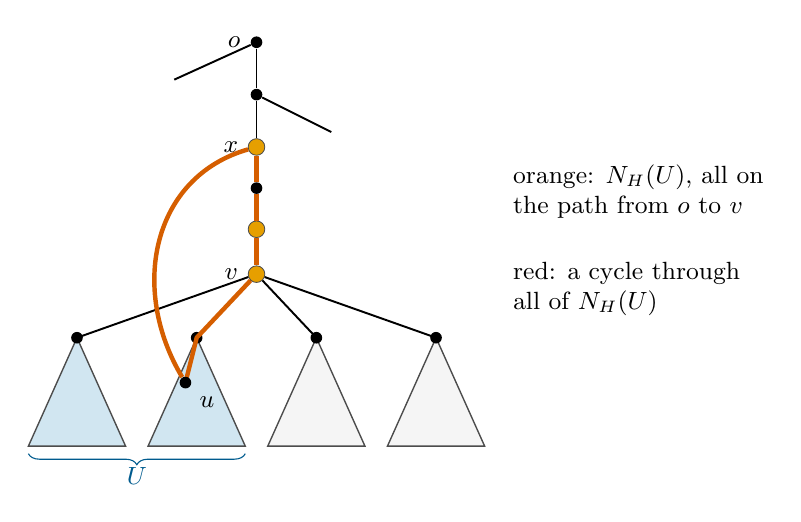
\begin{tikzpicture}[scale=.95]
  \node[vtx,label={[lbl]left:$o$}] (o) at (0,4.2) {};
  \node[vtx] (a1) at (0,3.5) {};
  \node[hub,label={[lbl]left:$x$}] (x) at (0,2.8) {};
  \node[vtx] (a2) at (0,2.25) {};
  \node[hub] (a3) at (0,1.7) {};
  \node[hub,label={[lbl]left:$v$}] (v) at (0,1.1) {};
  \draw[line width=.7pt] (o)--(a1)--(x);
  \draw[line width=1.6pt,cDel] (x)--(a2)--(a3)--(v);
  \draw[line width=.7pt] (a1) -- (1.0,3.0);
  \draw[line width=.7pt] (o) -- (-1.1,3.7);
  % subtrees
  \foreach \xx/\fl in {-2.4/1,-0.8/1,0.8/0,2.4/0}{
    \ifnum\fl=1
      \filldraw[draw=black!70,fill=cPort!18,line width=.5pt] (\xx,0.25) -- (\xx-0.65,-1.2) -- (\xx+0.65,-1.2) -- cycle;
    \else
      \filldraw[draw=black!70,fill=black!4,line width=.5pt] (\xx,0.25) -- (\xx-0.65,-1.2) -- (\xx+0.65,-1.2) -- cycle;
    \fi
    \node[vtx] at (\xx,0.25) {};
    \draw[line width=.7pt] (v) -- (\xx,0.25);
  }
  \draw[line width=1.6pt,cDel] (v) -- (-0.8,0.25) -- (-0.95,-0.35);
  \node[vtx,label={[lbl]below right:$u$}] (u) at (-0.95,-0.35) {};
  \draw[line width=1.6pt,cDel] (u) .. controls (-1.7,0.9) and (-1.4,2.4) .. (x);
  \node[lbl,cPort!80!black] at (-1.6,-1.6) {$U$};
  \draw[decorate,decoration={brace,amplitude=4pt,mirror},cPort!80!black] (-3.05,-1.3) -- (-0.15,-1.3);
  \node[lbl,align=left,anchor=west] at (3.3,2.2) {orange: $\NN_H(U)$, all on\\the path from $o$ to $v$};
  \node[lbl,align=left,anchor=west] at (3.3,0.9) {red: a cycle through\\all of $\NN_H(U)$};
\end{tikzpicture}
\caption{Proof of \cref{lem:longcycle}. In a depth-first search tree there are
no edges between different subtrees of $v$. So the external neighbourhood of
the shaded union $U$ of subtrees lies on the path from the root $o$ to $v$, and
the highest neighbour $x$ closes a cycle through all of it.}
\label{fig:dfs}
\end{figure}

\subsection{Splitting into expanders}\label{sec:splitting}

A graph that is not an $s$-expander has a set $U$ with a small external
neighbourhood once at most $s|U|$ edges are deleted. Such a set splits the graph
into two smaller graphs that overlap only in a small separator. Repeating this
gives a decomposition into expanders. This is the method of Buci\'c and
Montgomery~\cite[Lemma~14]{BM}. Coffey~\cite{Cof} added a rule that moves
vertices with many deleted edges into the separator. This makes the deleted
edges a thin cut, which is property~\ref{it:split-thin} below; it is what later
keeps the crowding of anchors small (\cref{lem:bookkeeping}\ref{it:bk-crowd}).

\begin{lemma}[A splitting step]\label{lem:split}
Let $s\ge0$ and $\tau>0$, and let $H$ be a graph on $N\ge2$ vertices which is
not an $s$-expander, with $\tau\ge256s\log^2N$. Then there is a partition
$V(H)=A\sqcup B\sqcup C$ with $A\ne\varnothing$ such that
\begin{enumerate}[label=\textup{(\roman*)},itemsep=1pt]
\item\label{it:split-shape} $|B|\le2\eps|A|/\log^2N$ and $|A|+|B|<3N/4$;
\item\label{it:split-del} the set $F=E_H(A,C)$ of \emph{deleted edges} satisfies
$|F|\le2s|A|$, and $F=\varnothing$ if $s=0$;
\item\label{it:split-thin} every vertex of $A$ has fewer than $\tau$ neighbours in
$C$, and every vertex of $C$ has fewer than $\tau$ neighbours in $A$.
\end{enumerate}
\end{lemma}

The two \emph{children} of $H$ are
\[
H_1=H[A\cup B]\qquad\text{and}\qquad H_2=H[B\cup C]-E(H[B]).
\]
They meet in the \emph{separator} $B$, both have fewer than $N$ vertices, and
$E(H)$ is the disjoint union of $E(H_1)$, $E(H_2)$ and $F$ (\cref{fig:split}).

\begin{proof}
Choose $U$ and $F'$ with $1\le|U|\le2N/3$, $|F'|\le s|U|$ and
$|\NN_{H-F'}(U)|<\eps|U|/\log^2N$. Let $S=\NN_{H-F'}(U)$ and
$C'=V(H)\setminus(U\cup S)$. All edges between $U$ and $C'$ lie in $F'$, so
$F_0=E_H(U,C')$ has at most $s|U|$ edges. Let $U^+$ be the set of vertices
$u\in U$ with $\deg_{F_0}(u)\ge\tau$, and let $A=U\setminus U^+$. Let $C^+$ be
the set of vertices of $C'$ with at least $\tau$ neighbours in $A$. Put
\[
B=S\cup U^+\cup C^+,\qquad C=C'\setminus C^+.
\]
The edges of $F_0$ at vertices of $U^+$ and the edges between $C^+$ and $A$ are
disjoint subsets of $F_0$. Hence $\tau(|U^+|+|C^+|)\le s|U|$, and so
$|U^+|+|C^+|\le|U|/(256\log^2N)=\eps|U|/(8\log^2N)$. Thus
$|A|\ge\frac{255}{256}|U|>0$ and
\[
|B|<\frac{9\eps|U|}{8\log^2N}\le\frac{2\eps|A|}{\log^2N},\qquad
|A|+|B|\le|U|+|B|\le\tfrac23N\bigl(1+\tfrac{9}{256}\bigr)<\tfrac34N.
\]
Every edge between $A\subseteq U$ and $C\subseteq C'$ lies in $F_0$, so
$|F|\le s|U|\le2s|A|$. If $s=0$ then $F_0=\varnothing$. Finally, a vertex of
$A$ has $\deg_{F_0}<\tau$, and a vertex of $C$ has fewer than $\tau$ neighbours
in $A$ by the definition of $C^+$.
\end{proof}

\begin{figure}[t]
\centering
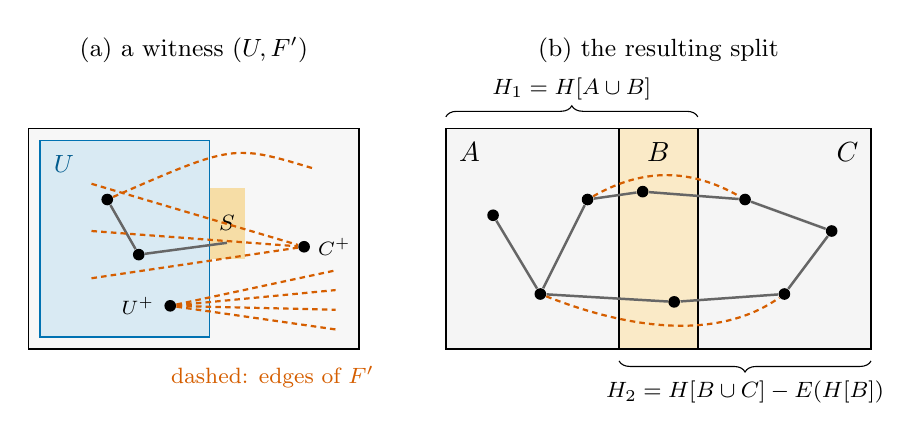
\begin{tikzpicture}[scale=1]
  % ---------------- panel (a): the witness
  \begin{scope}
    \node[lbl] at (2.1,3.8) {(a) a witness $(U,F')$};
    \draw[line width=.6pt,fill=black!3] (0,0) rectangle (4.2,2.8);
    \fill[cPort!15] (0.15,0.15) rectangle (2.3,2.65);
    \draw[cPort,line width=.6pt] (0.15,0.15) rectangle (2.3,2.65);
    \node[lbl,cPort!80!black] at (0.45,2.35) {$U$};
    \fill[cHub!35] (2.3,1.15) rectangle (2.75,2.05);
    \node[font=\footnotesize] at (2.52,1.6) {$S$};
    % U^+ vertices (high deleted degree)
    \node[vtx] (up) at (1.8,0.55) {};
    \node[font=\scriptsize,anchor=east] at (1.72,0.55) {$U^+$};
    \foreach \yy in {0.25,0.5,0.75,1.0}{\draw[del] (up) -- (3.9,\yy);}
    \node[vtx] (u1) at (1.0,1.9) {};
    \node[vtx] (u2) at (1.4,1.2) {};
    \draw[del] (u1) .. controls (2.6,2.6) .. (3.6,2.3);
    \draw[edg,black!60] (u2) -- (2.52,1.35);
    \draw[edg,black!60] (u1) -- (u2);
    \node[vtx] (cp) at (3.5,1.3) {};
    \node[font=\scriptsize,anchor=west] at (3.55,1.3) {$C^+$};
    \foreach \yy in {0.9,1.5,2.1}{\draw[del] (0.8,\yy) -- (cp);}
    \node[font=\footnotesize,cDel] at (3.1,-0.35) {dashed: edges of $F'$};
  \end{scope}
  % ---------------- panel (b): the split
  \begin{scope}[shift={(5.3,0)}]
    \node[lbl] at (2.7,3.8) {(b) the resulting split};
    \fill[black!4] (0,0) rectangle (2.2,2.8);
    \fill[cHub!22] (2.2,0) rectangle (3.2,2.8);
    \fill[black!4] (3.2,0) rectangle (5.4,2.8);
    \draw[line width=.6pt] (0,0) rectangle (5.4,2.8);
    \draw[line width=.6pt] (2.2,0)--(2.2,2.8) (3.2,0)--(3.2,2.8);
    \node at (0.3,2.5) {$A$};
    \node at (2.7,2.5) {$B$};
    \node at (5.1,2.5) {$C$};
    \foreach \n/\x/\y in {a1/0.6/1.7,a2/1.2/0.7,a3/1.8/1.9,b1/2.5/2.0,b2/2.9/0.6,c1/3.8/1.9,c2/4.3/0.7,c3/4.9/1.5}{
      \node[vtx] (\n) at (\x,\y) {};
    }
    \draw[edg,black!60] (a1)--(a2)--(a3)--(b1) (a2)--(b2)--(c2)--(c3)--(c1)--(b1);
    \draw[del] (a3) .. controls (2.5,2.3) and (3.1,2.3) .. (c1);
    \draw[del] (a2) .. controls (2.6,0.15) and (3.6,0.2) .. (c2);
    \draw[decorate,decoration={brace,amplitude=4pt}] (0,2.95) -- (3.2,2.95);
    \node[font=\footnotesize] at (1.6,3.3) {$H_1=H[A\cup B]$};
    \draw[decorate,decoration={brace,amplitude=4pt,mirror}] (2.2,-0.15) -- (5.4,-0.15);
    \node[font=\footnotesize] at (3.8,-0.55) {$H_2=H[B\cup C]-E(H[B])$};
  \end{scope}
\end{tikzpicture}
\caption{A splitting step (\cref{lem:split}). (a)~After deleting the dashed
edges $F'$, the set $U$ has only the small boundary $S$. Some vertices would be
left with many deleted edges: $U^+$ inside $U$, and $C^+$ outside it. (b)~These
vertices are moved into the separator $B=S\cup U^+\cup C^+$. The children
$H_1$ and $H_2$ overlap only in $B$, and edges inside $B$ go to $H_1$. The
deleted edges are now only the few edges between $A$ and $C$, and they form a
thin cut: no vertex has $\tau$ or more of them.}
\label{fig:split}
\end{figure}

A \emph{splitting tree} for a graph $H_0$ is a rooted binary tree whose nodes
are graphs and whose root is $H_0$. Each node $H$ that is not a leaf is split by
\cref{lem:split}, for some parameters $s_H,\tau_H$ such that $H$ is not an
$s_H$-expander and $\tau_H\ge256s_H\log^2|H|$. Its two children are the two
children of the split. The edge set of $H_0$ is the disjoint union of the edge
sets of the leaves and the sets of deleted edges at all splits.

Every vertex of a node lies in some leaf below it, because the children of a
node cover its vertex set. A vertex lies in two or more leaves if and only if it
lies in the separator of some split. Indeed, a vertex of a separator lies in
both children, and a vertex lying in two leaves lies in both children of their
lowest common ancestor. Such vertices are \emph{shared}, and the others are
\emph{private}. For a leaf $Y$ we write $\sh(Y)$ for its set of shared vertices.
A private vertex of $Y$ lies in exactly the nodes on the path from the root to
$Y$.

\begin{lemma}[Splitting trees]\label{lem:tree}
Let $\cT$ be a splitting tree for a graph $H_0$ on $n_0$ vertices.
\begin{enumerate}[label=\textup{(\alph*)},itemsep=1pt]
\item\label{it:tree-overlap} The leaves of $\cT$ have total order less than
$4n_0/3$.
\item\label{it:tree-shared} For every $\gamma\ge2$, $\sum_Y|\sh(Y)|<n_0/\log\gamma$,
where the sum is over the leaves $Y$ with $|Y|\ge\gamma$.
\item\label{it:tree-del} If $s_H\le s$ for every split, then at most
$7sn_0\log n_0$ edges are deleted in total.
\item\label{it:tree-thin} Suppose that $\tau_H\le\tau$ at every split that deletes
at least one edge. Then for every leaf $Y$ and every vertex $h$, fewer than
$\tau$ deleted edges join $h$ to private vertices of $Y$, and none do if
$h\in Y$.
\end{enumerate}
\end{lemma}

\begin{proof}
For every split of a node $H$, with parts $A,B,C$, and every $a\in A$, choose a
leaf below the first child that contains $a$, and call the pair (leaf, $a$) a
\emph{copy}. Consider a fixed copy $(Y,v)$, and let $H^{(1)}\supsetneq
H^{(2)}\supsetneq\dots$ be the nodes whose splits chose it. Each $H^{(i+1)}$
lies below the first child of $H^{(i)}$, so $|H^{(i+1)}|<\frac34|H^{(i)}|$.
Consequently, if all these nodes have order at least $\gamma\ge2$, then the
$j$-th smallest has order at least $\gamma(4/3)^{j-1}$.

\ref{it:tree-overlap},\ref{it:tree-shared} Let $\Sigma_\gamma$ be the sum of
$|B|$ over the splits of nodes of order at least $\gamma$. Spread the bound
$|B|\le\sum_{a\in A}2\eps/\log^2|H|$ of \cref{lem:split} over the copies chosen
at the split. A copy then receives at most
\[
2\eps\sum_{j\ge0}\frac1{(\log\gamma+j\log\frac43)^2}
\le2\eps\Bigl(\frac1{\log^2\gamma}+\frac1{\log\frac43\cdot\log\gamma}\Bigr)
<\frac{7\eps}{\log\gamma}
\]
from splits of order at least $\gamma$. Replacing a node by its two children
increases the total order by $|B|$, so the total order of the leaves is
$S=n_0+\Sigma_2$. As there are at most $S$ copies,
$\Sigma_\gamma<7\eps S/\log\gamma$. For $\gamma=2$ this gives $S<n_0+7\eps S$,
so $S<n_0/(1-7\eps)<4n_0/3$, which proves~\ref{it:tree-overlap}. Hence
$\Sigma_\gamma<\frac{7}{24}n_0/\log\gamma$.

For~\ref{it:tree-shared}, let $c_v$ be the number of leaves of order at least
$\gamma$ in which $v$ is shared, and $k_v$ the number of splits of nodes of
order at least $\gamma$ with $v$ in the separator. We claim $c_v\le2k_v$.
Suppose $c_v\ge1$. The leaves counted by $c_v$, together with their ancestors,
form a subtree whose nodes all have order at least $\gamma$ and contain $v$. If
$c_v\ge2$, this subtree has at least $c_v-1$ nodes with two children in it, and
$v$ lies in the separator of each of them. If $c_v=1$, then $v$ also lies in
another leaf, and $v$ lies in the separator of the lowest common ancestor of
the two leaves, which has order at least $\gamma$. Thus
$\sum_Y|\sh(Y)|=\sum_vc_v\le2\Sigma_\gamma<n_0/\log\gamma$.

\ref{it:tree-del} Spread the bound $|F|\le2s|A|$ over the copies chosen at the
split, $2s$ each. The orders of the nodes charging a fixed copy decrease by a
factor $3/4$ and lie between $2$ and $n_0$, so there are at most
$1+\log_{4/3}(n_0/2)\le2.41\log n_0$ of them. Hence at most
$2s\cdot\frac43n_0\cdot2.41\log n_0\le7sn_0\log n_0$ edges are deleted.

\ref{it:tree-thin} Let $hy$ be a deleted edge with $y$ private to $Y$, deleted
at the split of a node $H$. Since $y$ is private, $H$ is an ancestor of $Y$, and
$y$ lies in the part ($A$ or $C$) of the child towards $Y$. So $h$ lies in the
other part and not in the child towards $Y$, and therefore $h\notin Y$.
Moreover, $H$ is the last node on the path from the root to $Y$ that contains
$h$. So all the deleted edges in question are deleted at the same split. Since
$h$ and the private vertices of $Y$ lie in opposite parts of this split, there
are fewer than $\tau$ of them by \cref{lem:split}\ref{it:split-thin}.
\end{proof}

\subsection{The rounds}\label{sec:rounds}

We fix a large absolute constant $D$. Every statement from now on holds if $D$
is larger than a suitable absolute constant, and we assume this tacitly. We
write $\oD$ for any quantity bounded by $\eta(D)\,n$, where $\eta$ is a function
that depends only on $D$ and tends to $0$ as $D\to\infty$.

For a real number $d\ge D$ we use the parameters
\[
\lambda=\log d,\qquad M=\lceil d^2\rceil,\qquad s=\lceil\lambda^{50}\rceil,
\qquad \tau=\lceil\lambda^{53}\rceil,\qquad m=\lceil\lambda^{54}\rceil,
\]
with the meanings shown in \cref{tab:params}. The exponents are not optimised.
What matters are the relations between them, which are collected in
\cref{tab:requirements}: the pieces must be robust enough to lend reservoirs and
to clear vertices ($s$ large), the cut threshold must be compatible with the
splitting step but negligible compared with the pieces ($s\log^2M\ll\tau\ll m$),
and the next degree, about $s\lambda+m$, must still be polylogarithmic.

\begin{table}[h]
\centering\small
\begin{tabular}{@{}lll@{}}
\toprule
symbol & value & role\\
\midrule
$d_r$ & $2e(G_r)/n$ & average degree at the start of round $r$\\
$\lambda_r$, $\mu_r$ & $\log d_r$, $\log\lambda_r$ & logarithms of the degree\\
$M_r$ & $\lceil d_r^2\rceil$ & maximum order of a piece of round $r$\\
$s_r$ & $\lceil\lambda_r^{50}\rceil$ & pieces of round $r$ are $s_r$-expanders\\
$\tau_r$ & $\lceil\lambda_r^{53}\rceil$ & thin-cut threshold for splits in round $r$\\
$m_r$ & $\lceil\lambda_r^{54}\rceil$ & minimum order of a piece of round $r$\\
\bottomrule
\end{tabular}
\caption{The parameters of round $r$.}
\label{tab:params}
\end{table}

\begin{table}[h]
\centering\small
\renewcommand{\arraystretch}{1.15}
\begin{tabular}{@{}p{0.42\textwidth}p{0.5\textwidth}@{}}
\toprule
requirement & where it is used\\
\midrule
$\tau\ge256s\log^2M$ & splitting steps of round $r$ are legal (\cref{lem:split})\\
$\frac{56}3s\log M+\frac43m\le\lambda^{55}$ & the next degree is $d_{r+1}\le\lambda_r^{55}$, see~\ref{it:H-degree}\\
$\tau/m\le2/\lambda$ and $\log m\ge\mu$ & hubs and crowding are summable over rounds (\cref{lem:bookkeeping})\\
$s/4\ge\log^{40}M$ & a piece can clear vertices with its own edges (\cref{lem:clear})\\
$s\lambda^{-4}\ge\lambda^{46}\gg M_\ell^{13}\log^{18}M$ for $\ell\ge r+2$ & lent edges link through sparse slots (\cref{lem:good})\\
$s\lambda^{-5}\gg M_\ell^{15}$ for $\ell\ge r+2$ & donor sets are large (\cref{lem:deficient})\\
$m\ge M_\ell$ for $\ell\ge r+2$ & bad anchors are rare compared with slots (\cref{lem:Omega})\\
\bottomrule
\end{tabular}
\caption{What the proof needs from the exponents. Here $\lambda=\lambda_r$,
$\mu=\mu_r$, and $M_\ell\le(55\mu_r)^{111}$ by \cref{lem:scales}; the last
three requirements hold because $\lambda_r=2^{\mu_r}$ is exponentially larger
than any fixed power of $\mu_r$.}
\label{tab:requirements}
\end{table}

\paragraph{Construction.} Let $G_1=G$. For $r=1,2,\dots$ let
$d_r=2e(G_r)/n$. If $d_r<D$ we stop and put $R=r-1$. Otherwise we carry out
round $r$, with the parameters of \cref{tab:params}:
\begin{enumerate}[label=(R\arabic*),leftmargin=3.2em,itemsep=2pt]
\item\label{it:R1} \emph{Long cycles.} Repeatedly remove from $G_r$ a cycle of
length at least $d_r\lambda_r^2$, as long as there is one. Let $\cC_r$ be the
set of removed cycles and $G_r'$ the remaining graph.
\item\label{it:R2} \emph{Splitting.} Build a splitting tree $\cT_r$ for $G'_r$ in
two stages. In the first stage, split every node with at least two vertices
that is not a $0$-expander, with $(s_H,\tau_H)=(0,\tau_r)$. The leaves of the
first stage are $0$-expanders or single vertices. In the second stage, split
every node of order at least $m_r$ that is not an $s_r$-expander, with
$(s_H,\tau_H)=(s_r,\tau_r)$. The leaves of order at least $m_r$ are
$s_r$-expanders and are called the \emph{pieces} of round $r$. For a piece $Y$
(a set of vertices) we write $H_Y$ for the leaf itself, an $s_r$-expander with
vertex set $Y$.
\item\label{it:R3} \emph{Assignment.} Assign every edge of every $H_Y$ to $Y$.
Then assign every other edge of $G'_r$ with both ends in some piece to one such
piece. Let $E_Y\supseteq E(H_Y)$ be the set of edges assigned to $Y$.
\item\label{it:R4} \emph{Next round.} $G_{r+1}$ consists of the edges of $G'_r$
that were not assigned, on the vertex set $V(G)$.
\end{enumerate}
We write $\cY_r$ for the set of pieces of round $r$, and $\sh_r(Y)$ for the
shared vertices of $Y\in\cY_r$ in $\cT_r$.

\begin{lemma}[The hierarchy]\label{lem:hierarchy}
For every round $r\le R$:
\begin{enumerate}[label=\textup{(H\arabic*)},leftmargin=3.2em,itemsep=1pt]
\item\label{it:H-size} every piece $Y\in\cY_r$ has $m_r\le|Y|\le M_r$;
\item\label{it:H-overlap} $\sum_{Y\in\cY_r}|Y|<4n/3$, so $|\cY_r|<4n/(3m_r)$; and
$\sum_{Y\in\cY_r}|\sh_r(Y)|<n/\log m_r$;
\item\label{it:H-cycles} $|\cC_r|\le n/(2\lambda_r^2)$;
\item\label{it:H-degree} $d_{r+1}\le\lambda_r^{55}$;
\item\label{it:H-sep} \emph{(separation)} for every $\ell>r$, no edge of
$G_\ell$ has both ends in a piece of round $r$;
\item\label{it:H-thin} \emph{(thin cuts)} for every $Y\in\cY_r$ and every vertex
$h$, fewer than $\tau_r$ edges of $G_{r+1}$ join $h$ to vertices of
$Y\setminus\sh_r(Y)$.
\end{enumerate}
Moreover, $E(G)$ is the disjoint union of the cycles in $\bigcup_r\cC_r$, the
sets $E_Y$ over all pieces of all rounds, and $E(G_{R+1})$, where
$e(G_{R+1})<Dn/2$. The graphs $H_Y$ over all pieces of all rounds are pairwise
edge-disjoint.
\end{lemma}

\begin{proof}
\ref{it:H-size} Let $W$ be a leaf of the first stage, a $0$-expander, and
suppose $|W|>M_r$. By \cref{lem:longcycle} and since $x/\log^2x$ is increasing
for $x\ge8$, $W$ contains a cycle of length at least
$M_r/(2^8\log^2M_r)\ge d_r^2/(2^{8}\cdot9\lambda_r^2)>d_r\lambda_r^2$. But
$W\subseteq G'_r$, which has no such cycle. So the first-stage leaves, and
hence all pieces, have order at most $M_r$.

\ref{it:H-overlap} This follows from \cref{lem:tree}\ref{it:tree-overlap}
and~\ref{it:tree-shared} with $\gamma=m_r$.

\ref{it:H-cycles} Each removed cycle has at least $d_r\lambda_r^2$ of the
$d_rn/2$ edges of $G_r$.

\ref{it:H-degree} Every edge of $G_{r+1}$ is deleted in $\cT_r$ or lies in a
leaf of order less than $m_r$. The first stage deletes nothing. Below each
first-stage leaf $W$ the second stage is a splitting tree in which
$s_H\le s_r$. So by \cref{lem:tree}\ref{it:tree-del} it deletes at most
$7s_r|W|\log M_r$ edges. The first-stage leaves have total order less than
$4n/3$, so at most $7s_r\cdot\frac43n(2\lambda_r+1)\le30\lambda_r^{51}n$ edges
are deleted. A leaf $K$ of order less than $m_r$ has fewer than $|K|m_r/2$
edges, and all leaves have total order less than $4n/3$. Hence
$d_{r+1}\le60\lambda_r^{51}+\frac43m_r\le\lambda_r^{55}$.

\ref{it:H-sep} Every edge of $G'_r$ with both ends in a piece of round $r$ was
assigned in~\ref{it:R3}, and $G_\ell\subseteq G_{r+1}$ for $\ell>r$.

\ref{it:H-thin} Let $hu\in E(G_{r+1})$ with $u\in Y\setminus\sh_r(Y)$. If $hu$
lay in a leaf of $\cT_r$, that leaf would contain $u$, so it would be $Y$, and
$hu$ would have been assigned to $Y$. So $hu$ is a deleted edge, and
\cref{lem:tree}\ref{it:tree-thin} applies with $\tau=\tau_r$.

The final statements follow from the construction, since $d_{R+1}<D$.
\end{proof}

\begin{lemma}[Scales]\label{lem:scales}
Let $\mu_r=\log\lambda_r$.
\begin{enumerate}[label=\textup{(\alph*)},itemsep=1pt]
\item\label{it:sc-halve} For $r<R$: $\lambda_{r+1}\le\lambda_r/2$,
$\mu_{r+1}\le\mu_r/2$ and $M_{r+1}\le M_r/2$. Also $\mu_R\ge\log\log D$ and
$M_R\ge D^2$.
\item\label{it:sc-two} For $3\le\ell\le R$ and $r\le\ell-2$:
$M_\ell\le(55\mu_{\ell-2})^{111}\le(55\mu_r)^{111}$, and $2^{\ell-r}\le\lambda_r$.
\item\label{it:sc-sum} For fixed $a>0$ and $k\ge0$,
$\sum_{r=1}^R(R-r+1)^k\mu_r^{-a}=O_{a,k}\bigl((\log\log D)^{-a}\bigr)$. The same
holds with $\mu_r$ replaced by $\lambda_r$, $m_r$ or $M_r$, which are larger.
\end{enumerate}
\end{lemma}

\begin{proof}
\ref{it:sc-halve} By~\ref{it:H-degree},
$\lambda_{r+1}\le55\log\lambda_r=55\mu_r\le\lambda_r/2$ and
$\mu_{r+1}\le\log(55\mu_r)\le\mu_r/2$, because $\mu_r\ge\log\log D$ is large.
Also $d_{r+1}\le\lambda_r^{55}\le d_r/2$, which gives $M_{r+1}\le M_r/2$.
\ref{it:sc-two} We have $M_\ell\le2d_\ell^2\le2\lambda_{\ell-1}^{110}
\le2(55\mu_{\ell-2})^{110}\le(55\mu_{\ell-2})^{111}$. By~\ref{it:sc-halve},
$\lambda_r\ge2^{\ell-r}\lambda_\ell\ge2^{\ell-r}$.
\ref{it:sc-sum} By~\ref{it:sc-halve}, $\mu_r\ge2^{R-r}\log\log D$, so the sum
is at most $(\log\log D)^{-a}\sum_{j\ge0}(j+1)^k2^{-aj}$.
\end{proof}

Part~\ref{it:sc-sum} is the main place where the number of rounds enters. It is
why no factor $\log^\star n$ appears: quantities charged once per round, or even
once per pair of rounds, are summable because the parameters grow like a tower
towards earlier rounds. Part~\ref{it:sc-two} is why anchors are taken two rounds
back: $M_{r+1}$ may be as large as $\lambda_r^{110}$, but $M_{r+2}$ is only
polylogarithmic in $\lambda_r$.

\subsection{Roles}\label{sec:roles}

\begin{definition}[Hubs, residents, ports and anchors]\label{def:roles}
Fix a round $\ell\le R$. A \emph{hub} of round $\ell$ is a vertex that lies in
at least two pieces of round $\ell$. Let $\Hub_\ell$ be the set of hubs. A
vertex that lies in exactly one piece $X$ of round $\ell$ is a \emph{resident}
of $X$. A resident $u$ is a \emph{port} if some piece of a round $r\le\ell-2$
contains $u$. In that case we fix one such piece and call it the \emph{anchor}
$\anc_\ell(u)$; this choice depends only on the hierarchy, not on any of the
random choices made later. A resident that is not a port is \emph{fresh}, and
$\Fresh_\ell$ is the set of fresh residents.
\end{definition}

For a piece $Y$ of round $r$ and a round $\ell\ge r+2$, the \emph{crowding} of
$Y$ in round $\ell$ is
\[
\kappa_{Y,\ell}=\max_{h\in V(G)}\bigl|\{u: u\text{ is a port of round }\ell
\text{ with }\anc_\ell(u)=Y\text{ and }hu\in E(G_\ell)\}\bigr|.
\]
Crowding measures how many cherries can share a centre. The number of cycles
needed to close the cherries of an anchor grows with its crowding
(\cref{lem:cherry}), so we need the crowding to be small on average. Let
$\nu_\ell$ be the number of pieces of rounds at most $\ell-2$, that is, the
number of possible anchors in round $\ell$.

\begin{lemma}[Bookkeeping]\label{lem:bookkeeping}
\leavevmode
\begin{enumerate}[label=\textup{(\alph*)},itemsep=1pt]
\item\label{it:bk-fresh} $\sum_\ell|\Fresh_\ell|\le2n$.
\item\label{it:bk-hub} $\sum_\ell\sum_{X\in\cY_\ell}|X\cap\Hub_\ell|=\oD$.
\item\label{it:bk-crowd} $\kappa_{Y,\ell}<\tau_r+|\sh_r(Y)|$ for $Y\in\cY_r$, and
$\sum_{\ell}\sum_{r\le\ell-2}\sum_{Y\in\cY_r}\kappa_{Y,\ell}=\oD$.
\item\label{it:bk-anc} $\nu_\ell\le3n/m_{\ell-2}$, and
$\sum_{\ell=3}^R\nu_\ell M_\ell=\oD$.
\item\label{it:bk-cyc} $\sum_r|\cC_r|=\oD$.
\end{enumerate}
\end{lemma}

\begin{proof}
\ref{it:bk-fresh} Let $r_0$ be the first round in which a vertex $u$ lies in a
piece. In every round $\ell\ge r_0+2$ in which $u$ is a resident, the piece of
round $r_0$ containing $u$ makes $u$ a port. So $u$ is fresh in at most the two
rounds $r_0$ and $r_0+1$.

\ref{it:bk-hub} A hub lies in two leaves of $\cT_\ell$, so
$X\cap\Hub_\ell\subseteq\sh_\ell(X)$. By~\ref{it:H-overlap} the inner sum is
less than $n/\log m_\ell\le n/(54\mu_\ell)$. Now sum using
\cref{lem:scales}\ref{it:sc-sum}.

\ref{it:bk-crowd} Let $u$ be a port of round $\ell$ with anchor $Y\in\cY_r$ and
$hu\in E(G_\ell)\subseteq E(G_{r+1})$. If $u\notin\sh_r(Y)$, there are fewer
than $\tau_r$ such $u$ for a fixed $h$, by the thin-cut
property~\ref{it:H-thin}. All other such $u$ lie in $\sh_r(Y)$. Summing over
$Y\in\cY_r$ with~\ref{it:H-overlap}, and then over the fewer than $R-r$ rounds
$\ell$, the total is at most
\[
\sum_r(R-r)\Bigl(\frac{4n}{3m_r}\tau_r+\frac{n}{\log m_r}\Bigr)
\le\sum_r(R-r)\Bigl(\frac{2}{\lambda_r}+\frac{1}{54\mu_r}\Bigr)n=\oD.
\]

\ref{it:bk-anc} By~\ref{it:H-overlap} and \cref{lem:scales}\ref{it:sc-halve},
$\nu_\ell<\sum_{r\le\ell-2}4n/(3m_r)\le3n/m_{\ell-2}$. By
\cref{lem:scales}\ref{it:sc-two},
$\nu_\ell M_\ell\le3n(55\mu_{\ell-2})^{111}/\lambda_{\ell-2}^{54}\le
n/\lambda_{\ell-2}$, and the sum is $\oD$ by \cref{lem:scales}\ref{it:sc-sum}.

\ref{it:bk-cyc} This follows from~\ref{it:H-cycles} and
\cref{lem:scales}\ref{it:sc-sum}.
\end{proof}

% =====================================================================
\section{Linking through sparse random sets}\label{sec:linking}
% =====================================================================

Every cycle we build through an expander is closed by a path through a sparse
random set of vertices. This section states that robust expanders support such
paths, for many pairs at once. First we note that a random sample of the edges
of an expander is again an expander.

\begin{lemma}[Sampling edges]\label{lem:sample}
Let $H$ be an $s$-expander on $N$ vertices, and let $0<p\le1$ with
$ps\ge100\log N$. Let $H_p$ be the random spanning subgraph of $H$ that
contains every edge independently with probability $p$. Then $H_p$ is a
$(ps/2)$-expander with probability at least $1-N^{-10}$.
\end{lemma}

\begin{proof}
Suppose $H_p$ is not a $(ps/2)$-expander. Then there are $U$ with
$1\le u=|U|\le2N/3$ and $F\subseteq E(H_p)$ with $|F|\le psu/2$ such that
$T=\NN_{H_p-F}(U)$ has fewer than $\eps u/\log^2N$ vertices. All edges of $H_p$
between $U$ and $V(H)\setminus(U\cup T)$ lie in $F$. On the other hand, $H$ has
more than $su$ edges between $U$ and $V(H)\setminus(U\cup T)$: otherwise
deleting them would leave the external neighbourhood of $U$ inside $T$, which
contradicts expansion. So for this pair $(U,T)$, at most $psu/2$ of more than
$su$ given edges survive in $H_p$. By \cref{lem:chernoff} this has probability
at most $e^{-psu/8}\le N^{-18u}$. There are at most $N^{2u}$ pairs $(U,T)$ with
$|U|=u$, since $|T|<u$. Hence the failure probability is at most
$\sum_{u\ge1}N^{-16u}\le N^{-10}$.
\end{proof}

The following lemma is the engine of the proof. Buci\'c and Montgomery proved it
for random sets of density $1/3$ and a fixed polylogarithmic
multiplicity~\cite[Theorem~16]{BM}. We need sparse random sets and arbitrary
multiplicity.

\begin{lemma}[Linking]\label{lem:link}
There is an absolute constant $C_*$ such that the following holds. Let $t\ge1$
and $0<\rho\le1/2$, let $H$ be an $s$-expander on $N$ vertices with
$s\ge C_*t\rho^{-3}\log^{18}N$, and let $V\subseteq V(H)$ be random, containing
every vertex independently with probability $\rho$. Then with probability at
least $1-N^{-3}$, $H$ links through $V$ with multiplicity~$t$.
\end{lemma}

Linking through $V$ implies linking through every superset of $V$. Hence the
lemma also applies if every vertex is included independently with probability
\emph{at least} $\rho$: a $\rho$-random set can be coupled inside such a set.

The proof is in \cref{app:linking}. It follows the strategy of~\cite{BM}, with
two simplifications: a single bounded-degree certificate replaces their
two-case analysis~\cite[Proposition~13]{BM}, and Haxell's theorem replaces the
hypergraph matching theorem of Aharoni and Haxell~\cite{AH}. Here is its
outline. Write $L=\log N$. A \emph{ball} of radius $k$ around a set $U$ is the
set of vertices of $V$ that can be reached from $U$ by a path through $V$ of
length at most $k$.
\begin{enumerate}[label=(\arabic*),itemsep=2pt]
\item \emph{Haxell reduces linking to one path at a time.} By
\cref{thm:haxell}, applied to the families of short paths joining each pair, it
suffices to show the following: for any set of demands and any set $S$ of
forbidden edges whose size is linear in the number of demands, some demand can
still be joined by a short path through $V$ in $H-S$.
\item \emph{Large balls give such a path.} If every set of $u$ vertices has a
ball of radius $k$ covering more than half of $V$, then among any $2u-1$
disjoint demands one can be joined by a path of length $O(kL)$. This halving
argument is~\cite[Proposition~8]{BM}.
\item \emph{Balls grow.} In an expander, a random $p$-subset of a set $W$ has
about $\alpha|W|$ neighbours outside $W$, where $\alpha=\eps/L^2$. A maximal
bounded-degree bipartite subgraph between $W$ and its complement certifies
this, and a Bernstein inequality makes it hold with very high probability.
Exposing $V$ in $k=O(L/\alpha)$ independent batches, the ball around a set
grows by a factor $1+\alpha/16$ per batch until it covers most of the graph.
\item \emph{Union bound.} The growth fails with probability $N^{-\Omega(|A|)}$
only if the starting set $A$ is \emph{well-expanding}, with $|\NN(A)|\ge\theta|A|$.
Every set contains a large well-expanding subset~\cite[Proposition~18]{BM}, so
this suffices.
\item \emph{Amplification.} Steps (3) and (4) tolerate only about $|U|/L^{O(1)}$
deleted edges, while step (1) needs tolerance of about $t|U|L^{O(1)}$. Split the
edges of $H$ at random into $K$ colours, each again an expander by
\cref{lem:sample}. Any set of deleted edges puts at most a $1/K$ fraction of
itself into some colour, and that colour alone provides the large ball.
\end{enumerate}
The requirement $s\ge C_*t\rho^{-3}L^{18}$ collects the losses: the
multiplicity $t$ and one factor $\rho^{-1}$ enter through step (1), two further
factors $\rho^{-1}$ through steps (3) and (4), where one batch of $V$ has density
only $\rho/O(L^3)$, and the powers of $L$ come from the sublinear expansion.

% =====================================================================
\section{Three decomposition lemmas}\label{sec:three}
% =====================================================================

This section proves the three local moves of the proof. They are stated without
reference to the hierarchy. In \cref{sec:proof} they are applied once per piece
(\cref{lem:clear}) and once per round (\cref{lem:cherry,lem:quotient}). In all
three, $\Delta$ denotes a bound on degrees; in the application it is $M_\ell$.

\subsection{Clearing a set of vertices}

\begin{lemma}[Clearing]\label{lem:clear}
There is an absolute constant $N_0$ such that the following holds. Let $O$ be
an $s$-expander with vertex set $X$, where $N=|X|\ge N_0$ and
$s\ge\log^{40}N$. Let $E\supseteq E(O)$ be a set of edges with both ends in
$X$, and let $P\subseteq X$. Then there is a set $O'\subseteq E(O)$ with
\[
f\bigl(E[P]\cup O'\bigr)\le101|P|.
\]
\end{lemma}

So all edges inside $P$ can be removed at a constant cost per vertex of $P$,
using some further edges of $O$. Every edge of $E\setminus(E[P]\cup O')$ has an
end outside $P$.

The proof uses a \emph{vortex}, a nested sequence of random sets
$P=P_0\supseteq P_1\supseteq\dots\supseteq P_k$ whose sizes halve. This device
comes from iterative absorption~\cite{BKLO}. At step $j$ we decompose all
remaining edges that touch the layer $\Lambda_j=P_j\setminus P_{j+1}$ into paths
(\cref{lem:lovasz}). We extend each path at both ends so that it ends in the
next level, and close it into a cycle by a connecting path through a random set
inside the next level (\cref{fig:clear}). Closing paths through
path-connecting random sets is the method of~\cite{BM}. Combining it with a
vortex is due to Coffey~\cite{Cof}. What survives all $k$ steps lives on the
tiny set $P_k$ and is decomposed by \cref{lem:egp}.

\begin{proof}
Let $L=\log N$, and assume $P\ne\varnothing$.

\emph{Outlets.} Let $a=\lceil L^6\rceil$ and $b=\lceil64aL^2\rceil=\lceil
2aL^2/\eps\rceil$. We claim that every vertex $w$ has a set $\Omega(w)$ of $a$
neighbours in $O$, its \emph{outlets}, such that every vertex is an outlet of
at most $b$ vertices. Form a bipartite graph. On the left are the ordered pairs
$(w,y)$ with $wy\in E(O)$. On the right, every vertex $y$ has $b$ \emph{load}
slots and every vertex $w$ has $\deg_O(w)-a\ge0$ \emph{spare} slots. Join
$(w,y)$ to the load slots of $y$ and to the spare slots of $w$. A matching that
covers the left side gives, for every $w$, at least $a$ pairs $(w,y)$ matched to
load slots, and we let $\Omega(w)$ consist of $a$ of these vertices $y$.

We check Hall's condition~\cite{Hal}. Let $\Psi$ be a set of pairs, let
$\Theta$ be the set of their second coordinates, and let $S$ be the set of $w$
that occur in more than $\deg_O(w)-a$ pairs of $\Psi$. Then
$|\Psi|\le(\text{spare slots})+a|S|$, so it suffices that $b|\Theta|\ge a|S|$.
This holds trivially if $S=\varnothing$. Otherwise every $w\in S$ has fewer
than $a$ neighbours outside $\Theta$. Take $S'\subseteq S$ with
$|S|/2\le|S'|\le2N/3$, and delete the at most $(a-1)|S'|\le s|S'|$ edges from
$S'$ to outside $\Theta$. Then the external neighbourhood of $S'$ lies in
$\Theta$, so $|\Theta|\ge\eps|S'|/L^2\ge\eps|S|/(2L^2)$, and $b|\Theta|\ge a|S|$.

\emph{The random vortex.} Let $k=\lfloor\log(L/6)\rfloor$, so that
$6/L\le2^{-k}<12/L$. Make the following independent random choices.
\begin{itemize}[leftmargin=2em,itemsep=1pt]
\item Colour every edge of $O$ uniformly with one of $2k+1$ colours: a
\emph{reserve} colour and \emph{connector} colours $(j,c)$, for $0\le j<k$ and
$c\in\{1,2\}$. Let $O^{\mathrm{res}}$ and $O_{j,c}$ be the colour classes.
\item Give every $v\in P$ a level $\lev(v)\in\{0,\dots,k\}$ with
$\Pr(\lev(v)\ge j)=2^{-j}$, and put $\lev(v)=k$ for $v\notin P$. Let
$U_j=\{v:\lev(v)\ge j\}$, $P_j=P\cap U_j$ and $\Lambda_j=P_j\setminus P_{j+1}$.
\item Give every vertex a label in $\{0,1,2\}$, with probabilities
$\frac12,\frac14,\frac14$. For $c\in\{0,1,2\}$ let $V_{j,c}$ be the set of
vertices of $U_{j+1}$ with label $c$.
\end{itemize}
Thus $V_{j,0}$ will receive the reserved edges, and $V_{j,1},V_{j,2}$ will
carry the connectors of the two phases. We claim that with positive
probability the following hold:
\begin{enumerate}[label=(V\arabic*),itemsep=1pt]
\item\label{it:V-link} every $O_{j,c}$ with $c\in\{1,2\}$ links through
$V_{j,c}$ with multiplicity $b+2$;
\item\label{it:V-res} for every $w\in P$ and $j<k$, at least four edges of
$O^{\mathrm{res}}$ join $w$ to $\Omega(w)\cap V_{j,0}$;
\item\label{it:V-size} $\sum_{j<k}|P_j|\le8|P|$ and $|P_k|\le48|P|/L$.
\end{enumerate}
By \cref{lem:sample}, each $O_{j,c}$ is an $s/(4k+2)$-expander with
probability at least $1-N^{-10}$. Every vertex lies in $V_{j,c}$ independently
with probability at least $2^{-k}/4\ge1/L$. So \cref{lem:link}, with
$t=b+2=O(L^8)$ and $\rho=1/L$, gives~\ref{it:V-link} with probability
$1-O(kN^{-3})$; it needs $s/(4k+2)\ge C_*(b+2)L^{21}$, which holds as
$s\ge L^{40}$. For \ref{it:V-res}, the number of such edges is a sum of
independent indicators, one for each $y\in\Omega(w)$, with mean at least
$a\cdot\frac1{2k+1}\cdot\frac6L\cdot\frac12\ge L^4$. So by \cref{lem:chernoff}
it is less than four with probability at most $e^{-L^4/3}$, and a union bound
over the $Nk$ pairs $(w,j)$ costs $o(1)$. For \ref{it:V-size}, the means are
$\sum_j2^{-j}|P|<2|P|$ and $2^{-k}|P|<12|P|/L$, so by Markov's inequality each
fails with probability less than $1/4$. Fix an outcome satisfying
\ref{it:V-link}--\ref{it:V-size}.

\emph{Step $j$, for $j=0,1,\dots,k-1$.} Let $E_j$ be the set of edges of $E[P]$
not used so far. We maintain that $E_j\subseteq E[P_j]$, which holds for
$j=0$. Let $F_j$ be the set of edges of $E_j$ that meet $\Lambda_j$.
\begin{enumerate}[label=(\arabic*),itemsep=2pt]
\item For every $w\in\Lambda_j$ use \ref{it:V-res} to \emph{reserve} four edges
of $O^{\mathrm{res}}$ from $w$ to distinct outlets in $V_{j,0}$, two for each
\emph{phase} $c\in\{1,2\}$. Remove the reserved edges from $F_j$ if they lie in
it.
\item Give every remaining edge of $F_j$ a phase $c$ such that $V_{j,c}$
contains neither of its ends. This is possible: one end lies in $\Lambda_j$,
which is disjoint from $U_{j+1}$, and the other end has only one label.
\item For each phase $c$, decompose the edges of phase $c$ by
\cref{lem:lovasz} into at most $|P_j|$ paths, with every vertex an end of at
most two of them. At every end $w\in\Lambda_j$ of such a path, append a
distinct phase-$c$ reserved edge of $w$. The result is a trail whose ends lie in
$U_{j+1}$, all of whose edges meet $\Lambda_j$, and which avoids $V_{j,c}$. Only
its two new end vertices can repeat a vertex. So cutting out closed subtrails
splits it into at most two cycles and at most one path $P'$ that joins its two
ends, if they differ. All cycles have length at least three, since the graph is
simple. The path $P'$ has length at least two, because each of its edges meets
$\Lambda_j$ and its ends do not.
\item For each phase $c$, join the two ends of every residual path $P'$ by a
path through $V_{j,c}$ in $O_{j,c}$, edge-disjointly, using~\ref{it:V-link}. A
vertex of $U_{j+1}$ is an end of at most $2$ phase-$c$ paths from the
decomposition, and it is the far end of at most one phase-$c$ reserved edge of
each $w$ that has it as an outlet. So it lies in at most $b+2$ pairs. Each
connector meets its residual path only at the ends, since its interior lies in
$V_{j,c}$, which the residual path avoids. As the residual path has length at
least two, the two together form a cycle even if the connector is a single
edge.
\item Pay for the unused reserved edges.
\end{enumerate}
The edges of $E_j$ that do not meet $\Lambda_j$ lie in $E[P_{j+1}]$. So after
we also remove the connector edges that lie in $E[P]$, the invariant
$E_{j+1}\subseteq E[P_{j+1}]$ holds.

\emph{No edge is used twice.} Step $j$ uses three kinds of edges: edges of
$F_j\subseteq E_j$, which are unused by definition; reserved edges $wy$ with
$w\in\Lambda_j$ and $y\in U_{j+1}$; and connector edges of colours $(j,1),(j,2)$.
Every connector edge has both ends in $U_{j+1}$, because its interior lies in
$V_{j,c}\subseteq U_{j+1}$ and so do the ends of residual paths. An earlier step
$i<j$ uses only edges that meet $\Lambda_i$ (its edges of $F_i$ and its
reserved edges) and connector edges of colours $(i,\cdot)$. Since $\Lambda_i$
is disjoint from $U_{i+1}\supseteq U_j$, none of these is a reserved or
connector edge of step $j$. Within step $j$, the connectors of one phase are
edge-disjoint, the two phases use different colours, and connector edges do not
meet $\Lambda_j$, so they are not in $F_j$.

\emph{The finish and the count.} After step $k-1$ the unused edges of $E[P]$
lie in $E[P_k]$. By \cref{lem:egp} and~\ref{it:V-size} they cost at most
$|P_k|(\log|P_k|+1)\le|P_k|(L+1)\le49|P|$ objects. Step $j$ produces at most
three cycles per path and pays for at most $4|\Lambda_j|$ reserved edges. So all
steps together cost at most $6\sum_j|P_j|+4|P|\le52|P|$ objects. The total is
at most $101|P|$, and $O'$ consists of all reserved edges and of the connector
edges that were used.
\end{proof}

\begin{figure}[t]
\centering
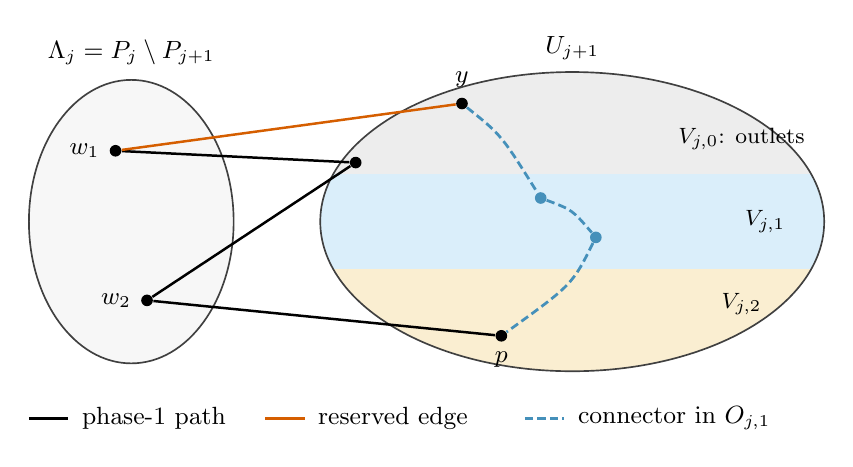
\begin{tikzpicture}[scale=1]
  \draw[piece] (0,0) ellipse (1.3 and 1.8);
  \node[lbl] at (0,2.15) {$\Lambda_j=P_j\setminus P_{j+1}$};
  \begin{scope}
    \clip (5.6,0) ellipse (3.2 and 1.9);
    \fill[black!7] (2,0.6) rectangle (9,2.2);
    \fill[cRes!22] (2,-0.6) rectangle (9,0.6);
    \fill[cHub!18] (2,-2.2) rectangle (9,-0.6);
  \end{scope}
  \draw[line width=.6pt,black!75] (5.6,0) ellipse (3.2 and 1.9);
  \node[lbl] at (5.6,2.2) {$U_{j+1}$};
  \node[font=\footnotesize] at (7.75,1.05) {$V_{j,0}$: outlets};
  \node[font=\footnotesize] at (8.05,0.0) {$V_{j,1}$};
  \node[font=\footnotesize] at (7.75,-1.05) {$V_{j,2}$};
  % path of phase 1, avoiding V_{j,1}
  \node[vtx,label={[lbl]left:$w_1$}] (w1) at (-0.2,0.9) {};
  \node[vtx] (p1) at (2.85,0.75) {};
  \node[vtx,label={[lbl]left:$w_2$}] (w2) at (0.2,-1.0) {};
  \node[vtx,label={[lbl]below:$p$}] (p2) at (4.7,-1.45) {};
  \draw[edg] (w1)--(p1)--(w2)--(p2);
  % reserved edge to an outlet
  \node[vtx,label={[lbl]above:$y$}] (y1) at (4.2,1.5) {};
  \draw[edg,cDel] (w1)--(y1);
  % connector through V_{j,1}
  \node[vtx,cRes!80!black] (c1) at (5.2,0.3) {};
  \node[vtx,cRes!80!black] (c2) at (5.9,-0.2) {};
  \draw[res] (y1) .. controls (4.7,1.1) .. (c1) .. controls (5.6,0.15) .. (c2) .. controls (5.6,-0.8) .. (p2);
  % legend
  \begin{scope}[shift={(-1.3,-2.5)}]
    \draw[edg] (0,0)--(0.5,0); \node[lbl,anchor=west] at (0.55,0) {phase-1 path};
    \draw[edg,cDel] (3.0,0)--(3.5,0); \node[lbl,anchor=west] at (3.55,0) {reserved edge};
    \draw[res] (6.3,0)--(6.8,0); \node[lbl,anchor=west] at (6.85,0) {connector in $O_{j,1}$};
  \end{scope}
\end{tikzpicture}
\caption{One step of the clearing lemma. A phase-1 path of remaining edges at
$\Lambda_j$ avoids $V_{j,1}$. Its end $w_1\in\Lambda_j$ is extended by a
reserved edge to an outlet $y\in V_{j,0}$. Its other end $p$ already lies in
$P_{j+1}$. The two ends, both in $U_{j+1}$, are joined by a connector through
$V_{j,1}$, which closes a cycle. Edges from $P_{j+1}$ to later levels are
handled in later steps.}
\label{fig:clear}
\end{figure}

\subsection{Closing cherries}

The second lemma chains cherries into cycles. In the application the ports are
the ports of one round, the classes are given by their anchors, and the
reservoirs are edges lent by the anchors.

\begin{lemma}[Cherries]\label{lem:cherry}
Let $E'$ be a set of edges and let $\Pi$ be a set of vertices, called
\emph{ports}, partitioned into classes $\Pi_Y$ indexed by a family $\cY$ of
vertex sets with $\Pi_Y\subseteq Y$. Let $\Delta,K\ge1$ be integers. Suppose
that:
\begin{enumerate}[label=\textup{(C\arabic*)},leftmargin=3em,itemsep=1pt]
\item\label{it:C1} every edge of $E'$ has an end in $\Pi$, and an edge of $E'$
at a port of $\Pi_Y$ has its other end outside $Y$;
\item\label{it:C2} every port is incident with at most $\Delta$ edges of $E'$;
\item\label{it:C3} for each $Y\in\cY$ there are pairwise disjoint sets
$T_{Y,1},\dots,T_{Y,K}\subseteq Y\setminus\Pi_Y$ and graphs
$R_{Y,1},\dots,R_{Y,K}$ with $V(R_{Y,j})\supseteq Y$ such that $R_{Y,j}$ links
through $T_{Y,j}$ with multiplicity $\Delta$;
\item\label{it:C4} the edge sets of all graphs $R_{Y,j}$ are pairwise disjoint
and disjoint from $E'$.
\end{enumerate}
For $Y\in\cY$ let $\kappa_Y=\max_x|\{u\in\Pi_Y:xu\in E'\}|$. Then there are
$J\subseteq E'$ and a set $R'$ of edges of the graphs $R_{Y,j}$ such that
$(E'\setminus J)\cup R'$ decomposes into at most
\[
\sum_{Y:\,\Pi_Y\neq\varnothing}\Bigl(\frac{\kappa_Y}2+2\Delta\Bigr)+\frac{|E'|}{2K}
\]
cycles, and for every $x\notin\Pi$ and every $Y$, at most one edge of $J$
joins $x$ to $\Pi_Y$.
\end{lemma}

\begin{proof}
Assign every edge of $E'$ to one of its ends in $\Pi$; edges at non-ports are
assigned to their port end. For an edge assigned to $u\in\Pi_Y$, call its other
end, which lies outside $Y$, its \emph{centre}, and call $Y$ its class. For
each class $Y$ and centre $x$, pair up the edges of class $Y$ with centre $x$
into \emph{cherries} $u\,x\,v$ with $u,v\in\Pi_Y$. If their number is odd, put
one of them into $J$. Every edge at a non-port $x$ has centre $x$, so $J$ has
the stated property.

Fix a class $Y$ with $N_Y$ cherries. Two cherries \emph{conflict} if they share
a vertex. A cherry $u\,x\,v$ conflicts with at most $\Delta-1$ others at each of
$u$ and $v$. Ends lie in $Y$ and centres do not, so a cherry can share $u$ or
$v$ only as an end. At the centre, a cherry conflicts with at most
$\kappa_Y/2-1$ others. So the conflict degree is at most $\kappa_Y/2+2\Delta-3$.
Put the cherries greedily into groups of at most $K$ pairwise vertex-disjoint
cherries, opening a new group only if every existing group is full or contains
a conflicting cherry. At most $\kappa_Y/2+2\Delta-3$ groups contain a
conflicting cherry, and fewer than $N_Y/K$ groups are full. So there are at most
$\kappa_Y/2+2\Delta-3+\lceil N_Y/K\rceil$ groups.

Order each group as $p_1x_1q_1,\dots,p_kx_kq_k$, with $k\le K$, and join $q_i$
to $p_{i+1}$ (indices modulo $k$) by a path through $T_{Y,i}$ in $R_{Y,i}$
(\cref{fig:cherries}). For each slot $i$, we request these connections for all
groups of class $Y$ at once. Each port is an end of at most $\Delta$ cherries,
so it lies in at most $\Delta$ requests for slot $i$, and \ref{it:C3} provides
edge-disjoint connectors. In a group, the connectors have their interiors in
the pairwise disjoint sets $T_{Y,i}\subseteq Y\setminus\Pi_Y$. These sets avoid
the ends of the cherries, which are ports of $\Pi_Y$, and the centres, which lie
outside $Y$. So each group becomes a cycle; when $k=1$ the cycle is $p_1x_1q_1$
followed by a connector from $q_1$ back to $p_1$. Different groups and
different classes use disjoint edges by~\ref{it:C4}. Since
$\sum_YN_Y\le|E'|/2$, summing the number of groups gives the bound.
\end{proof}

\begin{figure}[t]
\centering
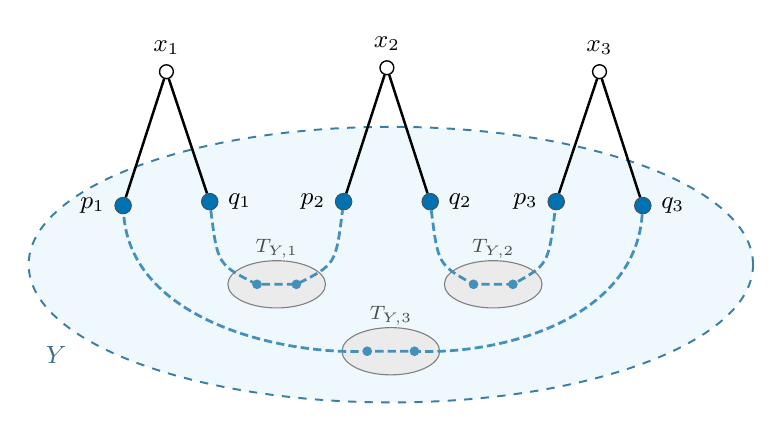
\begin{tikzpicture}[scale=1]
  \draw[ancr] (0,-0.2) ellipse (4.6 and 1.75);
  \node[lbl,cRes!60!black] at (-4.25,-1.35) {$Y$};
  \foreach \cx/\cy/\nm in {-1.45/-0.45/1,1.3/-0.45/2,0/-1.3/3}{
    \draw[black!50,fill=black!8] (\cx,\cy) ellipse (0.62 and 0.3);
    \node[font=\scriptsize,black!70] at (\cx,\cy+0.45) {$T_{Y,\nm}$};
  }
  \node[port,label={[lbl]left:$p_1$}] (p1) at (-3.4,0.55) {};
  \node[port,label={[lbl]right:$q_1$}] (q1) at (-2.3,0.6) {};
  \node[port,label={[lbl]left:$p_2$}] (p2) at (-0.6,0.6) {};
  \node[port,label={[lbl]right:$q_2$}] (q2) at (0.5,0.6) {};
  \node[port,label={[lbl]left:$p_3$}] (p3) at (2.1,0.6) {};
  \node[port,label={[lbl]right:$q_3$}] (q3) at (3.2,0.55) {};
  \node[plain,label={[lbl]above:$x_1$}] (x1) at (-2.85,2.25) {};
  \node[plain,label={[lbl]above:$x_2$}] (x2) at (-0.05,2.3) {};
  \node[plain,label={[lbl]above:$x_3$}] (x3) at (2.65,2.25) {};
  \draw[edg] (p1)--(x1)--(q1) (p2)--(x2)--(q2) (p3)--(x3)--(q3);
  \foreach \a/\b in {-1.7/-0.45,-1.2/-0.45,1.05/-0.45,1.55/-0.45,-0.3/-1.3,0.3/-1.3}{\node[vtx,cRes!80!black,minimum size=3.5pt] at (\a,\b) {};}
  \draw[res] (q1) .. controls (-2.2,-0.2) .. (-1.7,-0.45) -- (-1.2,-0.45) .. controls (-0.7,-0.2) .. (p2);
  \draw[res] (q2) .. controls (0.6,-0.2) .. (1.05,-0.45) -- (1.55,-0.45) .. controls (2.0,-0.2) .. (p3);
  \draw[res] (q3) .. controls (3.1,-0.9) and (1.4,-1.35) .. (0.3,-1.3) -- (-0.3,-1.3) .. controls (-1.4,-1.35) and (-3.3,-0.9) .. (p1);
\end{tikzpicture}
\caption{Closing a group of three vertex-disjoint cherries $p_ix_iq_i$ whose
ends lie in the anchor $Y$ and whose centres lie outside it. The connector from
$q_i$ to $p_{i+1}$ runs through its own slot $T_{Y,i}$, so the connectors are
internally disjoint from each other and from the cherries, and the result is
one cycle.}
\label{fig:cherries}
\end{figure}

\subsection{The quotient}

The third lemma turns the leftover edges into edges of an auxiliary graph whose
cycles lift to cycles of $G$. Leftovers are of two kinds: \emph{hub edges} $au$
from a hub $a$ to a port $u$, and \emph{links} $uv$ or $u\,x\,v$ between two
ports, possibly through a middle vertex $x$. Every end at a port is attached to
a pool vertex by a private \emph{donor} edge (\cref{fig:quotient}). Two things
must be controlled. First, the auxiliary graph must be simple. This is achieved
by splitting parallel edges into layers. Second, it must be small. Hubs are
grouped so that each hub has few copies, and the random choices of donors
spread the links evenly over the pools.

\begin{lemma}[Quotient]\label{lem:quotient}
Let $\Delta\ge2$, $g\ge4\Delta+4$ and $n\ge1$ be integers; $n$ only sets the
scale of the error term, and in our application it is $|V(G)|$. Let $A$, $\Pi$,
$I$, $W^-$ and $W^+$ be pairwise disjoint sets of vertices of a graph $\Gamma$
(hubs, ports, middles and two pools), and let $W=W^-\cup W^+$. Suppose we are
given:
\begin{itemize}[leftmargin=2em,itemsep=1pt]
\item a set $\cH$ of \emph{hub edges} $au$ with $a\in A$ and $u\in\Pi$, and a
set $\cL$ of \emph{links}, each an edge $uv$ or a path $u\,x\,v$ of $\Gamma$
with $u\ne v\in\Pi$ and $x\in I$, all edges involved being distinct;
\item every port lies on at most $\Delta$ hub edges and links, every middle lies
on at most $\Delta$ links, and $|\cH|,|\cL|\le n\Delta$;
\item for every port $u$, \emph{donor sets} $D^-(u)\subseteq\NN_\Gamma(u)\cap
W^-$ and $D^+(u)\subseteq\NN_\Gamma(u)\cap W^+$, each of size at least $g$;
\item a function $\beta:W\to\mathbb{Z}_{\ge0}$ such that for all $a\in A$ and
$w\in W$,
\begin{equation}\label{eq:beta}
\bigl|\{u: au\in\cH,\ w\in D^-(u)\cup D^+(u)\}\bigr|\le\beta(w).
\end{equation}
\end{itemize}
Then there are a set $\cH_\paid\subseteq\cH$ and a simple graph $Q$ with
\[
|\cH_\paid|+|V(Q)|\le|A|+\Delta^3\sum_{w\in W}\beta(w)
+3\Delta\lceil2\log\Delta\rceil|W|+30n\Bigl(\frac\Delta g+\frac1\Delta\Bigr),
\]
such that whenever $Q$ has a decomposition into $k$ objects, the set
$(\cH\setminus\cH_\paid)\cup E(\cL)\cup D'$ has a decomposition into at most $2k$
objects for some set $D'$ of \emph{donor edges} $uw$ with $w\in D^\pm(u)$.
\end{lemma}

Donor edges are never hub edges or edges of links, because $W$ is disjoint from
$A\cup\Pi\cup I$.

\begin{proof}
\emph{Layers.} Let $\cM$ be a loopless multigraph, and let $m(v,w)$ be the
number of edges between $v$ and $w$. Its \emph{layers} are the simple graphs
$\cM_1,\cM_2,\dots$, where $\cM_i$ contains the $i$-th edge of each parallel
class, and isolated vertices are removed. Their total number of vertices is
$\sum_v\max_wm(v,w)$.

\emph{The random choices.} The proof makes two kinds of independent random
choices: a colour for every group of hub edges (defined below), and, for every
port $u$, a pair of injections $\phi^-_u,\phi^+_u$. All other choices are
deterministic functions of these.

\emph{Hub edges.} For every hub $a$, split the hub edges at $a$ into groups of
size $\lfloor g/2\rfloor$, except for at most one smaller group. There are at
most $|A|+4|\cH|/g$ groups. Colour the groups independently and uniformly with
$\Delta^3$ colours, and give each hub edge the colour of its group. Let
$\cH_\paid$ be the set of hub edges $au$ for which another hub edge at $u$ has
the same colour. Two hub edges at $u$ come from different hubs, hence from
different groups, so $\Pr(au\in\cH_\paid)\le(\Delta-1)/\Delta^3$ and
$\E|\cH_\paid|\le|\cH|/\Delta^2\le n/\Delta$. For each hub edge
$au\notin\cH_\paid$ choose a donor $w(au)\in D^-(u)\cup D^+(u)$, by a fixed
greedy rule. The donors must be distinct for distinct hub edges at the same
port and for hub edges in the same group. This is possible, since fewer than
$\Delta+g/2\le g$ choices are excluded. For each colour $\gamma$, let
$\cM_\gamma$ be the multigraph with an edge $a\,w(au)$ for every hub edge
$au\notin\cH_\paid$ of colour $\gamma$. A group contributes at most one edge to
any pair $(a,w)$, so the copies of $a$ in the layers of all $\cM_\gamma$ number
at most the number of groups at $a$. Distinct hub edges at $a$ with the same
donor $w$ have distinct ports, so by~\eqref{eq:beta} every pool vertex $w$ has
at most $\beta(w)$ copies per colour. These layers therefore have at most
$|A|+4n\Delta/g+\Delta^3\sum_w\beta(w)$ vertices.

\emph{Links.} Colour the links greedily with at most $3\Delta$ colours so that
links of the same colour share no port and no middle; a link meets at most
$3(\Delta-1)$ others. Orient every link from one end port to the other. For
every port $u$, let $\phi^-_u$ be a uniformly random injection from the links
leaving $u$ into $D^-(u)$ minus the donors of hub edges at $u$, and let
$\phi^+_u$ be a uniformly random injection from the links entering $u$ into
$D^+(u)$ minus those donors. The domains have size at most $\Delta$, and the
ranges have size at least $g-\Delta\ge g/2$. A link from $u$ to $v$ thus gets
a \emph{tail junction} $w^-=\phi_u^-(\text{link})\in W^-$ and a \emph{head
junction} $w^+=\phi_v^+(\text{link})\in W^+$. For each colour $\gamma$, let
$\cN_\gamma$ be the multigraph with an edge $w^-w^+$ for every link of colour
$\gamma$, and split it into layers.

To bound the number of vertices we use an occupancy estimate. Let
$\xi_1,\dots,\xi_q$ be independent random variables, each taking every value
with probability at most $\pi$, and let $X_y=|\{i:\xi_i=y\}|$. Then for every
integer $t\ge1$
\begin{equation}\label{eq:occupancy}
\E\max_yX_y\le t+2e\pi q+4e2^{-t}q.
\end{equation}
Indeed, $\Pr(X_y\ge j)\le\E\binom{X_y}{j}\le(\E X_y)^j/j!\le(e\E X_y/j)^j$.
For $j\ge T=\max(t,\lceil2e\pi q\rceil)$ we have $e\E X_y/j\le1/2$, so this is
at most $(e\E X_y/j)2^{1-j}$, and summing gives
$\E[X_y\mathbf 1_{X_y\ge T}]\le4e2^{-T}\E X_y$. Now use
$\max_yX_y\le T-1+\sum_yX_y\mathbf1_{X_y\ge T}$ and $\sum_y\E X_y=q$.

Condition on the colours of the groups, which determine the hub donors and
hence the ranges of all injections, and on all the injections $\phi^-_u$,
which determine the tail junctions. The injections $\phi^+_v$ are still
independent and uniform. Fix a colour $\gamma$ and a pool vertex $w\in W^-$.
The links of colour $\gamma$ with tail junction $w$ have distinct head ports,
because links of one colour share no port. So their head junctions are
determined by different injections $\phi^+_v$. They are therefore independent,
and each is uniform on a set of size at least $g/2$. The number of copies of
$w$ in the layers of $\cN_\gamma$ is the maximum multiplicity of an edge at
$w$. By~\eqref{eq:occupancy} with $t=\lceil2\log\Delta\rceil$ and $\pi=2/g$, its
conditional expectation is at most $t+4eq_w/g+4eq_w/\Delta^2$, where $q_w$ is
the number of these links. The same holds for $w\in W^+$, conditioning on the
head junctions instead. Summing over $w$ and over the $3\Delta$ colours, the
expected number of vertices in the layers of all $\cN_\gamma$ is at most
$3\Delta t|W|+8en\Delta/g+8en/\Delta$.

\emph{The graph $Q$.} Let $Q$ be the vertex-disjoint union of all layers of all
$\cM_\gamma$ and $\cN_\gamma$. Adding up, $\E(|\cH_\paid|+|V(Q)|)$ is at most
the bound in the lemma, since $4+8e<30$ and $1+8e<30$. Fix an outcome of the
random choices that achieves this bound.

\emph{Lifting.} An edge $aw$ of $Q$ that comes from the hub edge $au$
\emph{represents} the path $a\,u\,w$, and an edge $w^-w^+$ that comes from a
link represents the path $w^-\,u\,v\,w^+$ or $w^-\,u\,x\,v\,w^+$. These paths
have three properties.
\begin{enumerate}[label=(L\arabic*),itemsep=1pt]
\item Distinct edges of $Q$ represent edge-disjoint paths. The hub edges and
links are distinct, and the donor edges at a port are distinct by construction:
hub donors are distinct, and the injections avoid them and map into the
disjoint sets $W^-$ and $W^+$.
\item In each layer, distinct vertices are distinct vertices of $\Gamma$. These
are hubs and pool vertices.
\item In each layer, the interior vertices of the represented paths are pairwise
distinct and are not vertices of the layer. In one colour a port lies on at
most one surviving hub edge, links of one colour share no port or middle, and
ports and middles are neither hubs nor pool vertices.
\end{enumerate}
Take a decomposition of $Q$ into $k$ objects. A cycle of $Q$ lies in one layer,
and by (L2) and (L3) replacing each of its edges by the represented path gives a
cycle of $\Gamma$. For a single edge of $Q$ we output only its \emph{core}: the
hub edge, or the one or two edges of the link. Its donor edges are left unused.
By (L1) this gives at most $2k$ edge-disjoint objects covering exactly
$(\cH\setminus\cH_\paid)\cup E(\cL)\cup D'$, where $D'$ is the set of donor
edges on lifted cycles.
\end{proof}

\begin{figure}[t]
\centering
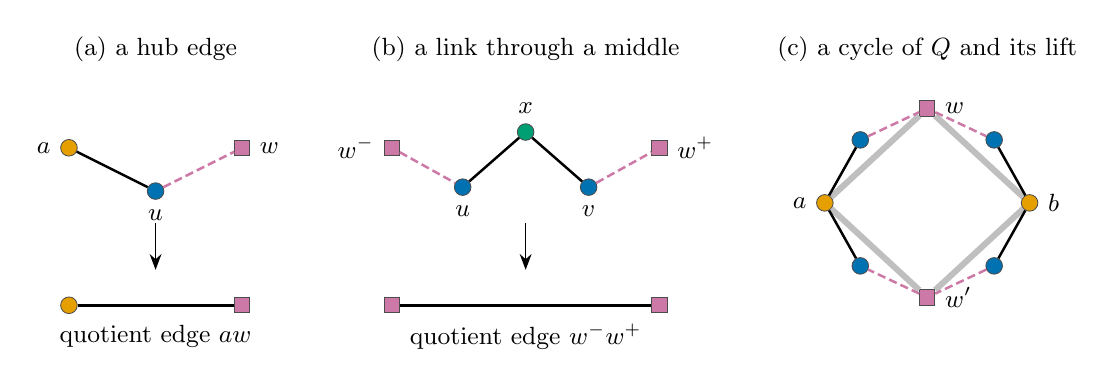
\begin{tikzpicture}[scale=1]
  % panel (a)
  \begin{scope}
    \node[hub,label={[lbl]left:$a$}] (a) at (0,0) {};
    \node[port,label={[lbl]below:$u$}] (u) at (1.1,-0.55) {};
    \node[pool,label={[lbl]right:$w$}] (w) at (2.2,0) {};
    \draw[edg] (a)--(u);
    \draw[edg,cPool,dash pattern=on 3pt off 1.5pt] (u)--(w);
    \draw[-{Stealth[length=2mm]},line width=.6pt] (1.1,-0.95)--(1.1,-1.55);
    \node[hub] (a') at (0,-2.0) {}; \node[pool] (w') at (2.2,-2.0) {};
    \draw[edg] (a')--(w');
    \node[lbl] at (1.1,-2.4) {quotient edge $aw$};
    \node[lbl] at (1.1,1.25) {(a) a hub edge};
  \end{scope}
  % panel (b)
  \begin{scope}[shift={(4.1,0)}]
    \node[pool,label={[lbl]left:$w^-$}] (wm) at (0,0) {};
    \node[port,label={[lbl]below:$u$}] (u) at (0.9,-0.5) {};
    \node[fresh,label={[lbl]above:$x$}] (x) at (1.7,0.2) {};
    \node[port,label={[lbl]below:$v$}] (v) at (2.5,-0.5) {};
    \node[pool,label={[lbl]right:$w^+$}] (wp) at (3.4,0) {};
    \draw[edg,cPool,dash pattern=on 3pt off 1.5pt] (wm)--(u);
    \draw[edg] (u)--(x)--(v);
    \draw[edg,cPool,dash pattern=on 3pt off 1.5pt] (v)--(wp);
    \draw[-{Stealth[length=2mm]},line width=.6pt] (1.7,-0.95)--(1.7,-1.55);
    \node[pool] (wm') at (0,-2.0) {}; \node[pool] (wp') at (3.4,-2.0) {};
    \draw[edg] (wm')--(wp');
    \node[lbl] at (1.7,-2.4) {quotient edge $w^-w^+$};
    \node[lbl] at (1.7,1.25) {(b) a link through a middle};
  \end{scope}
  % panel (c)
  \begin{scope}[shift={(10.9,-0.7)}]
    \node[hub,label={[lbl]left:$a$}] (a) at (-1.3,0) {};
    \node[hub,label={[lbl]right:$b$}] (b) at (1.3,0) {};
    \node[pool,label={[lbl]right:$w$}] (w) at (0,1.2) {};
    \node[pool,label={[lbl]right:$w'$}] (w2) at (0,-1.2) {};
    \node[port] (u1) at (-0.85,0.8) {};
    \node[port] (u2) at (0.85,0.8) {};
    \node[port] (u3) at (0.85,-0.8) {};
    \node[port] (u4) at (-0.85,-0.8) {};
    \draw[black!25,line width=2.2pt] (a)--(w)--(b)--(w2)--(a);
    \draw[edg] (a)--(u1) (b)--(u2) (b)--(u3) (a)--(u4);
    \draw[edg,cPool,dash pattern=on 3pt off 1.5pt] (u1)--(w)--(u2) (u3)--(w2)--(u4);
    \node[lbl] at (0,1.95) {(c) a cycle of $Q$ and its lift};
  \end{scope}
\end{tikzpicture}
\caption{The quotient. (a)~A hub edge $au$, extended by a donor edge $uw$
(dashed) to a pool vertex, becomes the edge $aw$ of $Q$. (b)~A link
$u\,x\,v$ between two ports becomes an edge between two pool vertices. (c)~The
cycle $a\,w\,b\,w'$ of $Q$ (grey) lifts to an $8$-cycle of $G$. The branch
vertices are hubs and pool vertices, and the private ports in between keep the
lift simple.}
\label{fig:quotient}
\end{figure}

% =====================================================================
\section{Proof of the reduction theorem}\label{sec:proof}
% =====================================================================

Let $G$ be a graph on $n$ vertices. If $2e(G)/n<D$ we pay for all edges, and
$f(G)<Dn/2$. Otherwise we build the hierarchy of \cref{sec:rounds}, with rounds
$1,\dots,R$, and use the notation of \cref{sec:hierarchy}.

\subsection{Plan}\label{sec:plan}

The proof has two phases.

\emph{Random preparation} (\cref{sec:random}). One random experiment, carried
out once for all pieces, does three things. It colours the edges of every
piece $Y$, so that $Y$ keeps half of its edges for itself and lends small
random slices to each later round. It chooses random \emph{slots} inside $Y$,
through which the lent edges will route. And it chooses sparse random
\emph{pools} of vertices for the quotients. A few ports are unlucky: their anchor
is bad, they fall into a slot of their anchor (\emph{lost} ports), or they have
too few donor edges (\emph{deficient} ports). One random variable $\Omega$
collects everything that such ports, and the pools, cost. Its expectation is
$\oD$, and we fix an outcome with $\Omega=\oD$.

\emph{Deterministic assembly} (\cref{sec:assembly}). We decompose the rounds in
the order $R,R-1,\dots,1$. Round $\ell$ starts from the edges assigned to its
pieces, minus the lent edges that later rounds have already used, and runs four
steps (\cref{fig:pipeline}). \Cref{lem:ledger} checks that every edge of $G$ is
used exactly once, and \cref{sec:count} adds up the costs.

\begin{figure}[t]
\centering
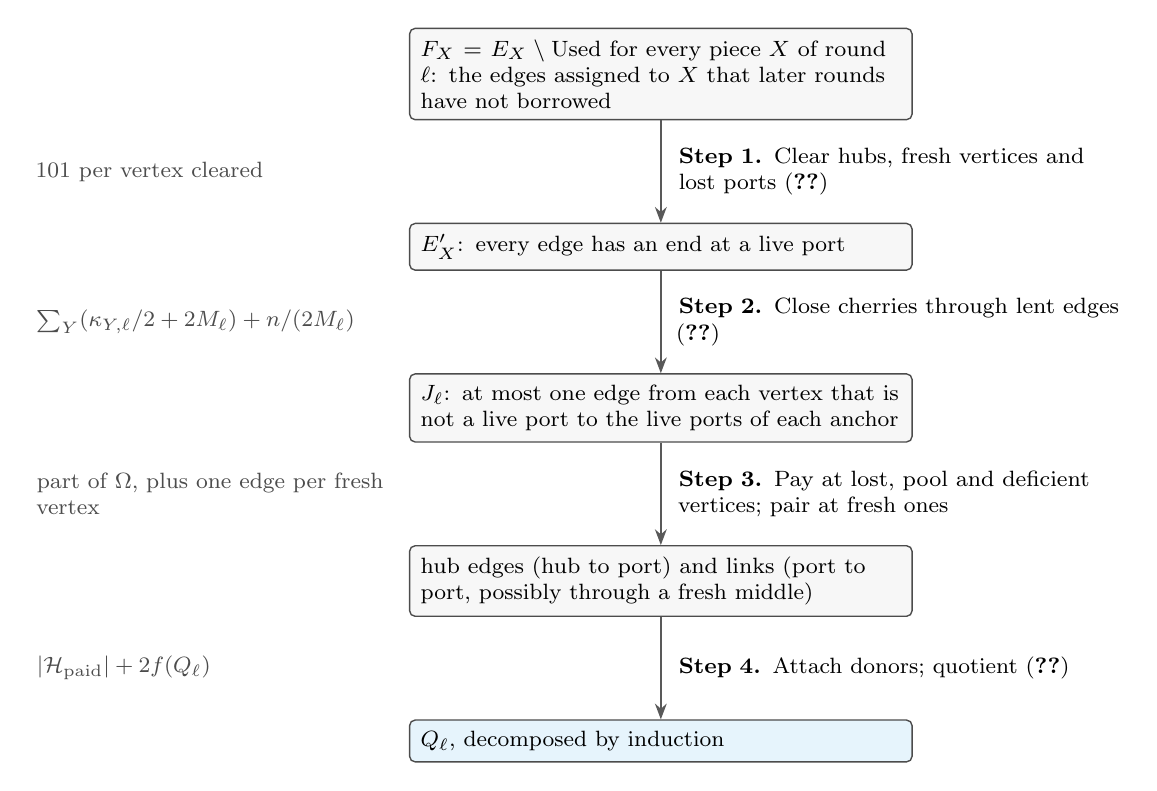
\begin{tikzpicture}[
  stage/.style={draw=black!70,line width=.5pt,rounded corners=2pt,fill=black!3,align=left,font=\footnotesize,inner sep=4pt,text width=6.1cm},
  stepnote/.style={font=\footnotesize,align=left,text width=5.6cm,text=black},
  costnote/.style={font=\footnotesize,align=left,text width=4.4cm,black!70},
  node distance=3.5mm]
  \node[stage] (s0) {$F_X=E_X\setminus\Used$ for every piece $X$ of round $\ell$:
  the edges assigned to $X$ that later rounds have not borrowed};
  \node[stage,below=13mm of s0] (s1) {$E'_X$: every edge has an end at a live
  port};
  \node[stage,below=13mm of s1] (s2) {$J_\ell$: at most one edge from each
  vertex that is not a live port to the live ports of each anchor};
  \node[stage,below=13mm of s2] (s3) {hub edges (hub to port) and links (port to
  port, possibly through a fresh middle)};
  \node[stage,fill=cRes!15,below=13mm of s3] (s4) {$Q_\ell$, decomposed by
  induction};
  \foreach \a/\b/\t/\c in {
    s0/s1/{\textbf{Step 1.} Clear hubs, fresh vertices and lost ports (\cref{lem:clear})}/{$101$ per vertex cleared},
    s1/s2/{\textbf{Step 2.} Close cherries through lent edges (\cref{lem:cherry})}/{$\sum_Y(\kappa_{Y,\ell}/2+2M_\ell)+n/(2M_\ell)$},
    s2/s3/{\textbf{Step 3.} Pay at lost, pool and deficient vertices; pair at fresh ones}/{part of $\Omega$, plus one edge per fresh vertex},
    s3/s4/{\textbf{Step 4.} Attach donors; quotient (\cref{lem:quotient})}/{$|\cH_\paid|+2f(Q_\ell)$}}{
    \draw[arr] (\a.south) -- (\b.north) node[midway,right=1mm,stepnote] {\t};
    \node[costnote,anchor=east] at ($(\a.south)!0.5!(\b.north)+(-3.4,0)$) {\c};
  }
\end{tikzpicture}
\caption{One round of the assembly. Boxes show the edges that remain after each
step. The text to the right of each arrow says what the step does, and the text
to the left says what it costs.}
\label{fig:pipeline}
\end{figure}

\paragraph{Where the costs go.} Only two things cost $\Theta(n)$: fresh
vertices, which are cleared and paired at most twice each, and the final sparse
graph $G_{R+1}$. Hubs, crowding, the number of anchors and $\Omega$ are summable
over the rounds by \cref{lem:scales}\ref{it:sc-sum}, so they cost $\oD$. The
quotients have $\oD$ vertices in total and are handled by induction.

\subsection{Random preparation}\label{sec:random}

\paragraph{Reservoirs.} Let $Y$ be a piece of round $r$. It lends to the rounds
$\ell\in\{r+2,\dots,R\}$, and for each such round it needs $M_\ell^2$ closing
colours and one donor colour. Put
\[
\chi_r=\sum_{\ell=r+2}^R(M_\ell^2+1).
\]
By \cref{lem:scales} we have $M_\ell\le M_{r+2}2^{-(\ell-r-2)}$ and
$M_{r+2}\le(55\mu_r)^{111}$, so $\chi_r\le3(55\mu_r)^{222}\le\lambda_r^4/2$.

\begin{definition}[Reservoirs]\label{def:reservoir}
Colour every edge of $H_Y$ independently at random. It gets the \emph{own}
colour with probability $1/2$. Each of the following colours has probability
$1/(2\chi_r)$: for every $\ell\in\{r+2,\dots,R\}$, the \emph{closing} colours
$(\ell,j)$ with $j\in[M_\ell^2]$, and the \emph{donor} colour $\ell$. If
$r+2>R$, all edges get the own colour. Let $O_Y$, $R_{Y,\ell,j}$ and
$\Rdon_{Y,\ell}$ be the spanning subgraphs of $H_Y$ formed by these colour
classes. Independently, for every $\ell$, give every vertex of $Y$ a
\emph{slot} for round $\ell$. It is slot $j$ with probability $M_\ell^{-4}$ for
each $j\in[M_\ell^2]$, and no slot otherwise. Let $T_{Y,\ell,j}$ be the set of
vertices with slot $j$ for round $\ell$. The piece $Y$ is \emph{good} if
\begin{enumerate}[label=(G\arabic*),itemsep=1pt]
\item\label{it:G1} $O_Y$ is an $(s_r/4)$-expander, and
\item\label{it:G2} every $R_{Y,\ell,j}$ links through $T_{Y,\ell,j}$ with
multiplicity $M_\ell$.
\end{enumerate}
Otherwise it is \emph{bad}.
\end{definition}

\begin{lemma}\label{lem:good}
Every piece $Y$ is bad with probability at most $|Y|^{-2}$.
\end{lemma}

\begin{proof}
Let $N=|Y|$, so $\lambda_r^{54}\le N\le M_r$ and $\log N\le3\lambda_r$. By
\cref{lem:sample} with $p=1/2$, \ref{it:G1} fails with probability at most
$N^{-10}$. Each $R_{Y,\ell,j}$ is a random subgraph with
$p=1/(2\chi_r)\ge\lambda_r^{-4}$, so by \cref{lem:sample} it is a
$(\lambda_r^{46}/2)$-expander with probability at least $1-N^{-10}$. The set
$T_{Y,\ell,j}$ is $M_\ell^{-4}$-random and independent of the colouring.
\Cref{lem:link} with $t=M_\ell$ and $\rho=M_\ell^{-4}$ needs
$\lambda_r^{46}/2\ge C_*M_\ell^{13}(3\lambda_r)^{18}$, which holds since
$M_\ell\le(55\mu_r)^{111}$. So~\ref{it:G2} fails for a given $(\ell,j)$ with
probability at most $N^{-10}+N^{-3}$. There are at most
$\chi_r\le\lambda_r^4\le N^{1/10}$ pairs $(\ell,j)$, so the total failure
probability is at most $N^{-2}$.
\end{proof}

\begin{definition}[Lost and live ports]\label{def:lost}
A port $u$ of round $\ell$ with anchor $Y=\anc_\ell(u)$ is \emph{lost} if $Y$ is
bad or $u$ lies in some slot set $T_{Y,\ell,j}$. Otherwise it is \emph{live}.
Let $\Lost_\ell$ be the set of lost ports of round $\ell$.
\end{definition}

So a live port avoids all slot sets of its anchor for its round, as
\cref{lem:cherry} requires, and its anchor is good. If a piece is bad, every
port anchored at it in every round is lost, so a bad piece never lends
anything.

\paragraph{Pools.} Independently of all previous choices, give every vertex of
$G$ at most one \emph{pool label} $(\ell,r,\sigma)$, with $3\le\ell\le R$,
$1\le r\le\ell-2$ and $\sigma\in\{-,+\}$. Each label has probability
$q_\ell2^{-(\ell-r)}$, where $q_\ell=M_\ell^{-5}$. The total probability is at
most $\sum_\ell q_\ell<1$. Let $W_{\ell,r,\sigma}$ be the set of vertices with
label $(\ell,r,\sigma)$, let $W_\ell^\sigma=\bigcup_rW_{\ell,r,\sigma}$ and
$W_\ell=W_\ell^-\cup W_\ell^+$, and for $w\in W_\ell$ let $r(w)$ be the second
coordinate of its label. Every vertex lies in $W_\ell$ with probability less
than $q_\ell$.

The pool of round $\ell$ is split by the round $r$ of the anchors it serves.
The reason is condition~\eqref{eq:beta} of \cref{lem:quotient}: a pool vertex
$w$ may serve as a donor for ports with many different anchors, but only
anchors of one round $r(w)$, and these anchors all contain $w$. The weights
$2^{-(\ell-r)}$ make the resulting cost summable over $r$ (\cref{lem:Omega}).

\paragraph{Donors.} Let $u$ be a port of round $\ell$ with anchor $Y$ of round
$r$. Its donor sets are
\[
D^\sigma(u)=\NN_{\Rdon_{Y,\ell}}(u)\cap W_{\ell,r,\sigma}\qquad(\sigma\in\{-,+\}).
\]
Let $g_\ell=M_\ell^{10}$. The port $u$ is \emph{deficient} if
$|D^-(u)|<g_\ell$ or $|D^+(u)|<g_\ell$. Let $\Def_\ell$ be the set of deficient
ports of round $\ell$.

\begin{lemma}\label{lem:deficient}
Every port of round $\ell$ is deficient with probability at most
$2e^{-g_\ell}$.
\end{lemma}

\begin{proof}
For a fixed $\sigma$, $|D^\sigma(u)|$ is a sum of independent indicators, one
for each of the more than $s_r$ neighbours $w$ of $u$ in $H_Y$: the edge $uw$
has the donor colour $\ell$, and $w\in W_{\ell,r,\sigma}$. By
\cref{lem:scales}\ref{it:sc-two}, $2^{\ell-r}\le\lambda_r$ and
$M_\ell\le(55\mu_r)^{111}$, so the mean is at least
\[
\lambda_r^{50}\cdot\lambda_r^{-4}\cdot M_\ell^{-5}2^{-(\ell-r)}
\ge\lambda_r^{45}M_\ell^{-5}\ge4M_\ell^{10}=4g_\ell.
\]
By \cref{lem:chernoff} it is less than $g_\ell$ with probability at most
$e^{-g_\ell}$.
\end{proof}

\Cref{tab:random} summarises the random choices. They are all independent, and
they are made after the hierarchy and the anchors have been fixed.

\begin{table}[h]
\centering\small
\renewcommand{\arraystretch}{1.15}
\begin{tabular}{@{}p{0.33\textwidth}p{0.3\textwidth}p{0.29\textwidth}@{}}
\toprule
object & distribution & purpose\\
\midrule
own graph $O_Y\subseteq H_Y$ & each edge with probability $\frac12$ & clearing inside $Y$ (\cref{lem:clear})\\
closing graphs $R_{Y,\ell,j}$, $j\in[M_\ell^2]$ & each edge with probability $\frac1{2\chi_r}$ & closing cherries in round $\ell$ (\cref{lem:cherry})\\
donor graph $\Rdon_{Y,\ell}$ & each edge with probability $\frac1{2\chi_r}$ & donor edges in round $\ell$ (\cref{lem:quotient})\\
slot sets $T_{Y,\ell,j}\subseteq Y$ & each vertex with probability $M_\ell^{-4}$ & interiors of cherry connectors\\
pools $W_{\ell,r,\pm}\subseteq V(G)$ & each vertex with probability $q_\ell2^{-(\ell-r)}$ & vertices of the quotient $Q_\ell$\\
\bottomrule
\end{tabular}
\caption{The random choices for a piece $Y$ of round $r$ and a later round
$\ell\ge r+2$, and for the pools. Lost and deficient ports are the ports for
which these choices fail.}
\label{tab:random}
\end{table}

\paragraph{The random cost.} Let $\Eas_\ell=\bigcup_{X\in\cY_\ell}E_X$ be the
set of edges assigned in round $\ell$. Every resident has fewer than $M_\ell$
edges in $\Eas_\ell$, because its piece has at most $M_\ell$ vertices. For a hub
$h$ of round $\ell$, let $c_\ell(h)$ be the number of anchors $Y$ such that some
edge of $\Eas_\ell$ joins $h$ to a port with anchor $Y$. Let
\[
\omega_\ell(v)=\begin{cases}c_\ell(v)&\text{if }v\in\Hub_\ell,\\
M_\ell&\text{otherwise.}\end{cases}
\]
Let $\beta_r(w)$ be the number of pieces of round $r$ that contain $w$, and let
$t_\ell=\lceil2\log M_\ell\rceil$. The \emph{random cost} is
\[
\Omega=\sum_{\ell=3}^R\Bigl[\underbrace{(101+M_\ell)|\Lost_\ell|}_{\text{lost ports}}
+\underbrace{\sum_{v\in W_\ell}\omega_\ell(v)}_{\text{pool vertices}}
+\underbrace{M_\ell|\Def_\ell|}_{\text{deficient ports}}
+\underbrace{M_\ell^3\!\!\sum_{w\in W_\ell}\!\beta_{r(w)}(w)+3M_\ell t_\ell|W_\ell|}_{\text{size of }Q_\ell}\Bigr].
\]
The first term pays for clearing lost ports (Step 1) and for their remaining
edges (Step 3). The second and third pay for the edges at pool vertices and at
deficient ports (Step 3). The last two bound the size of the quotient
(Step 4).

The weights $\omega_\ell$ deserve a comment. In Step 3 we pay for the leftover
edges at pool vertices. The leftover graph is produced by Step 2, which runs
after the pools are fixed, so its degrees at pool vertices are not independent
of the pools. But these degrees are bounded by the deterministic weights
$\omega_\ell$ (see Step 3), and a sum of deterministic weights over a random set
is easy to control.

\begin{lemma}\label{lem:Omega}
$\E\Omega=\oD$.
\end{lemma}

\begin{proof}
Fix $\ell\ge3$. A port $u$ with anchor $Y$ of round $r\le\ell-2$ has
$|Y|\ge m_r\ge M_\ell$, so $\Pr(u\in\Lost_\ell)\le|Y|^{-2}+M_\ell^2\cdot
M_\ell^{-4}\le2M_\ell^{-2}$ by \cref{lem:good}. Hence
$\E(101+M_\ell)|\Lost_\ell|\le4n/M_\ell$. Every pair $(h,Y)$ counted by
$c_\ell(h)$ is witnessed by a distinct edge of $\Eas_\ell$ at a port, so
$\sum_v\omega_\ell(v)\le2nM_\ell$, and therefore
$\E\sum_{v\in W_\ell}\omega_\ell(v)\le2n/M_\ell^4$. By \cref{lem:deficient},
$\E M_\ell|\Def_\ell|\le2nM_\ell e^{-g_\ell}\le n/M_\ell$. Since
$\sum_w\beta_r(w)=\sum_{Y\in\cY_r}|Y|<4n/3$,
\[
\E\sum_{w\in W_\ell}\beta_{r(w)}(w)=\sum_{r\le\ell-2}2q_\ell2^{-(\ell-r)}
\sum_w\beta_r(w)\le\tfrac43nq_\ell,
\]
so the fourth term has expectation at most $2n/M_\ell^2$. The last term has
expectation at most $3M_\ell t_\ell q_\ell n\le n/M_\ell$. Altogether
$\E\Omega\le\sum_\ell10n/M_\ell\le20n/D^2$ by
\cref{lem:scales}\ref{it:sc-halve}.
\end{proof}

We fix an outcome of all the random choices with $\Omega\le\E\Omega$. From now
on everything is deterministic. All that the rest of the proof uses about this
outcome is the definitions of good, live and deficient, and the bound
$\Omega=\oD$.

\subsection{Decomposing the rounds in reverse order}\label{sec:assembly}

We process the rounds $\ell=R,R-1,\dots,1$ in this order, and keep a set
$\Used$ of lent edges that the rounds processed so far have used. It is
initially empty. Round $\ell$ consists of the following four steps.

\paragraph{Step 1: clear.} For every piece $X$ of round $\ell$, let
$F_X=E_X\setminus\Used$, and let
\[
P_X=X\cap(\Hub_\ell\cup\Fresh_\ell\cup\Lost_\ell).
\]
Let $O_X$ be the own graph of $X$ if $X$ is good, and $O_X=H_X$ if $X$ is bad.
Apply \cref{lem:clear} to $O=O_X$, $E=F_X$ and $P=P_X$, and let
$E'_X=F_X\setminus(F_X[P_X]\cup O')$ be the set of edges of $F_X$ that remain.

\emph{Legitimacy.} We need $O_X\subseteq F_X$, that is, no edge of $O_X$ has
been used by a later round. Later rounds use only lent colours. If $X$ is good,
$O_X$ consists of own-coloured edges. If $X$ is bad, every port anchored at $X$
is lost, so no cherry of class $X$ is ever closed and no donor set of $X$ is
ever used; hence no edge of $X$ is in $\Used$. Moreover $O_X$ is an
$(s_\ell/4)$-expander with $s_\ell/4\ge(3\lambda_\ell)^{40}\ge\log^{40}|X|$, and
$|X|\ge m_\ell\ge N_0$.

\emph{Outcome.} Every vertex of $X$ is a hub, a fresh vertex, a lost port or a
live port, so every edge of $E'_X$ has an end at a live port. For $\ell\le2$
there are no ports, so $P_X=X$, $E'_X=\varnothing$, and the round ends here.

\emph{Cost.} At most $101|P_X|$ objects.

\paragraph{Step 2: close cherries} ($\ell\ge3$). Let $E'=\bigcup_XE'_X$. Apply
\cref{lem:cherry} to $E'$, with the live ports of round $\ell$ as ports,
classified by their anchors, and with $\Delta=M_\ell$, $K=M_\ell^2$,
$T_{Y,j}=T_{Y,\ell,j}$ and $R_{Y,j}=R_{Y,\ell,j}$. Add the lent edges used to
$\Used$, and let $J_\ell$ be the leftover set.

\emph{Legitimacy.} \ref{it:C1}: Let $u$ be a live port with anchor $Y$ of round
$r$, and let $uy\in E'\subseteq E(G_\ell)$. By the separation
property~\ref{it:H-sep}, $y\notin Y$. \ref{it:C2}: $u$ has fewer than $M_\ell$
edges in $E_X$. \ref{it:C3}: The anchor $Y$ of a live port is good, so the
graphs $R_{Y,\ell,j}$, which span $Y$, link through $T_{Y,\ell,j}$
by~\ref{it:G2}. The sets $T_{Y,\ell,j}$ are pairwise disjoint and avoid the live
ports anchored at $Y$. The colours $(\ell,j)$ are used only in round $\ell$, so
none of these edges is in $\Used$. \ref{it:C4}: The graphs $H_Y$ are pairwise
edge-disjoint, and they are disjoint from $E'\subseteq\Eas_\ell$.

\emph{Outcome.} $J_\ell$ has at most one edge between each vertex that is not a
live port and the live ports of each anchor.

\emph{Cost.} Every edge of $E'$ has a live port as an end, and every port has
fewer than $M_\ell$ edges in $\Eas_\ell$, so $|E'|\le nM_\ell$. Since
$\kappa_Y\le\kappa_{Y,\ell}$ and at most $\nu_\ell$ anchors occur, the number of
cycles is at most
\[
\sum_Y\Bigl(\frac{\kappa_{Y,\ell}}2+2M_\ell\Bigr)+\frac n{2M_\ell},
\]
where $Y$ runs over the pieces of rounds at most $\ell-2$.

\paragraph{Step 3: pay.} Pay for every edge of $J_\ell$ with an end in
$\Lost_\ell\cup W_\ell\cup\Def_\ell$. Then, at every fresh vertex $x\notin
W_\ell$, pair up the remaining edges of $J_\ell$ at $x$ into links $u\,x\,v$,
and pay for the leftover edge if their number is odd. Since $J_\ell$ is simple,
$u\ne v$.

\emph{Cost.} All edges of $J_\ell$ lie in $\Eas_\ell$, so a vertex that is not a
hub has $J_\ell$-degree less than $M_\ell$. Every edge of $J_\ell$ at a hub $h$
ends at a live port, because every edge of $E'$ has a live-port end and hubs are
not ports. So by the outcome of Step 2, $h$ has $J_\ell$-degree at most
$c_\ell(h)$. Hence, whatever $J_\ell$ is, the edges paid for at pool vertices
number at most $\sum_{v\in W_\ell}\omega_\ell(v)$, and those paid for at lost and
deficient ports number at most $M_\ell(|\Lost_\ell|+|\Def_\ell|)$. At most one
edge is paid for at each fresh vertex.

\paragraph{Step 4: quotient.} Apply \cref{lem:quotient} with $\Gamma=G$,
$\Delta=M_\ell$ and $g=g_\ell$. The hubs are $A=\Hub_\ell\setminus W_\ell$, the
ports $\Pi$ are the live ports outside $W_\ell\cup\Def_\ell$, the middles are
$I=\Fresh_\ell\setminus W_\ell$, the pools are $W^\pm=W_\ell^\pm$, and the donor
sets are $D^\pm(u)$. The hub edges are the remaining edges of $J_\ell$ between
$A$ and $\Pi$. The links are the remaining edges of $J_\ell$ inside $\Pi$,
together with the paths formed in Step~3. Finally,
$\beta(w)=\beta_{r(w)}(w)$. Pay for the edges of $\cH_\paid$. Take a
decomposition of $Q_\ell$ into $f(Q_\ell)$ objects, lift it, and add the donor
edges used to $\Used$.

\emph{Legitimacy.} The sets $A$, $\Pi$, $I$, $W^-$ and $W^+$ are pairwise
disjoint, since hubs, ports and fresh vertices are different roles and the pools
were removed from the first three. After Step 3, every edge of $J_\ell$ has a
port in $\Pi$ as one end. Its other end is a hub in $A$, a port in $\Pi$, or a
fresh vertex in $I$, because all other cases were paid for in Step~3. So the
remaining edges are exactly the hub edges and the edges of links. Ports lie on
fewer than $M_\ell$ of these, middles on fewer than $M_\ell/2$ links, and there
are at most $nM_\ell$ of each kind. The donor sets have size at least
$g_\ell\ge4M_\ell+4$, because the ports in $\Pi$ are not deficient, and the
donor colour $\ell$ is used only in round $\ell$. For
condition~\eqref{eq:beta}, let $au$ be a hub edge and $w\in D^\pm(u)$. Then the
anchor of $u$ is a piece of round $r(w)$ that contains $w$. Distinct such
ports $u$ have distinct anchors, because $J_\ell$ has at most one edge from $a$
to the live ports of each anchor. So there are at most $\beta_{r(w)}(w)$ of
them.

\emph{Cost.} At most $|\cH^\ell_\paid|+2f(Q_\ell)$ objects, where
\begin{equation}\label{eq:Qsize}
|\cH^\ell_\paid|+|V(Q_\ell)|\le|\Hub_\ell|+M_\ell^3\!\!\sum_{w\in W_\ell}\!\beta_{r(w)}(w)
+3M_\ell t_\ell|W_\ell|+30n\Bigl(\frac1{M_\ell^9}+\frac1{M_\ell}\Bigr).
\end{equation}

\begin{lemma}[Every edge is used exactly once]\label{lem:ledger}
The long cycles, the single edges of $G_{R+1}$, and the objects produced in
Steps 1--4 of all rounds form a decomposition of $E(G)$.
\end{lemma}

\begin{proof}
By \cref{lem:hierarchy}, $E(G)$ is partitioned into the long cycles, the edges
of $G_{R+1}$, and the sets $E_X$ for all pieces $X$. Fix a piece $X$ of round
$\ell$. Every edge of $E_X$ in a lent colour is used by at most one object,
namely in its target round $\ell'\ge\ell+2$, which is processed before round
$\ell$; when this happens it is added to $\Used$. Every other edge of $E_X$, and
every lent edge of $X$ that was not used, lies in $F_X$ when round $\ell$
starts. Within round $\ell$, the edges of $F_X$ are used exactly once: Step 1
uses $F_X[P_X]\cup O'$, and passes the rest, $E'_X$, to Step 2; Step 2 uses
$E'\setminus J_\ell$ and passes $J_\ell$ on; Step 3 pays for some edges of
$J_\ell$ and passes the rest on as hub edges and links; and Step 4 covers these
exactly once by \cref{lem:quotient}. The other edges used in round $\ell$ are
lent edges of earlier pieces, in colours $(\ell,j)$ and $\ell$; each of them is
used at most once, by \cref{lem:cherry,lem:quotient}, and is then added to
$\Used$, so it is not used again when its owner is processed.
\end{proof}

\subsection{Counting}\label{sec:count}

\Cref{tab:costs} lists all objects produced. Clearing costs at most
$101\sum_\ell\sum_X|P_X|$, and
\[
\sum_X|P_X|\le\sum_X|X\cap\Hub_\ell|+|\Fresh_\ell|+|\Lost_\ell|,
\]
since fresh and lost vertices are residents. The other entries follow from the
costs of Steps~2--4, \cref{lem:bookkeeping}, $\Omega=\oD$ and
\cref{lem:scales}\ref{it:sc-sum}.

\begin{table}[h]
\centering\small
\renewcommand{\arraystretch}{1.15}
\begin{tabular}{@{}p{0.43\textwidth}lp{0.3\textwidth}@{}}
\toprule
objects & number & reason\\
\midrule
long cycles $\cC_r$ & $\oD$ & \cref{lem:bookkeeping}\ref{it:bk-cyc}\\
single edges of $G_{R+1}$ & $<Dn/2$ & \cref{lem:hierarchy}\\
clearing hubs & $\oD$ & \cref{lem:bookkeeping}\ref{it:bk-hub}\\
clearing fresh vertices & $\le202n$ & \cref{lem:bookkeeping}\ref{it:bk-fresh}\\
clearing lost ports; paying at lost, pool and deficient vertices & first three terms of $\Omega$ & Steps 1 and 3\\
cherry cycles & $\oD$ & \cref{lem:bookkeeping}\ref{it:bk-crowd},\ref{it:bk-anc} and \cref{lem:scales}\ref{it:sc-sum}\\
unpaired edges at fresh vertices & $\le2n$ & \cref{lem:bookkeeping}\ref{it:bk-fresh}\\
paid hub edges in the quotients & $\oD$ & \eqref{eq:Qsize}, see below\\
lifted decompositions & $\le2\sum_\ell f(Q_\ell)$ & \cref{lem:quotient}\\
\bottomrule
\end{tabular}
\caption{The cost of the decomposition. Only fresh vertices, at most twice
each, and the final sparse graph cost $\Theta(n)$. Everything charged to rounds
is summable.}
\label{tab:costs}
\end{table}

Summing~\eqref{eq:Qsize} over $\ell$, the first term is $\oD$ by
\cref{lem:bookkeeping}\ref{it:bk-hub}, the next two are the last two terms of
$\Omega$, and the last is $\oD$ by \cref{lem:scales}\ref{it:sc-sum}. So
\begin{equation}\label{eq:Qtotal}
\sum_\ell\bigl(|\cH^\ell_\paid|+|V(Q_\ell)|\bigr)=\oD.
\end{equation}

\begin{proof}[Proof of \cref{thm:reduction}]
Choose $D$ so large that all requirements above hold and that the left side
of~\eqref{eq:Qtotal}, together with all entries $\oD$ of \cref{tab:costs}, is at
most $n/4$. By \cref{lem:ledger} the objects produced form a decomposition of
$E(G)$, so $\sum_\ell|V(Q_\ell)|\le n/4$ and
\[
f(G)\le\Bigl(\frac D2+202+2+\frac14\Bigr)n+2\sum_\ell f(Q_\ell).
\]
So \cref{thm:reduction} holds with $C_0=D/2+205$. The constant $D$, and hence
$C_0$, is absolute, because every requirement on $D$ involves only absolute
constants.
\end{proof}

% =====================================================================
\section{Sources}\label{sec:sources}
% =====================================================================

Every ingredient of the proof is listed here with its source. Numbers of
results in~\cite{BM} refer to its arXiv version.

\begin{itemize}[leftmargin=2em,itemsep=3pt]
\item \emph{Classical tools.} \Cref{lem:egp} is the classical $O(n\log n)$
argument. \Cref{lem:lovasz} is Lov\'asz's theorem~\cite{Lov} in the form
of~\cite[Corollary~22]{BM}. \Cref{thm:haxell} is Haxell's theorem~\cite{Hax}.
The probabilistic tools are standard~\cite{JLR,Fre,McD}, and Hall's
theorem~\cite{Hal} is used in \cref{lem:clear}.
\item \emph{Expanders.} Sublinear expanders are due to Koml\'os and
Szemer\'edi~\cite{KS1,KS2}, and their robust form to Haslegrave, Kim and
Liu~\cite{HKL} and Sudakov and Tomon~\cite{ST}. \Cref{def:expander} is
\cite[Definition~11]{BM}.
\item \emph{Rounds.} The overall scheme of rounds with long-cycle removal,
splitting into expanders and polylogarithmic decay of the degree is that of
Buci\'c and Montgomery~\cite{BM}, including the splitting step
(\cite[Lemma~14]{BM}) and the use of long cycles in expanders
(\cite[Lemma~25]{BM}). The depth-first-search proof of \cref{lem:longcycle} is
a standard argument (see~\cite{Kri}) and is shorter than the one in~\cite{BM}.
\item \emph{Thin cuts.} The rule that moves high-degree vertices into the
separator (\cref{lem:split}\ref{it:split-thin},
\cref{lem:tree}\ref{it:tree-thin}) and its use to bound crowding
(\cref{lem:bookkeeping}\ref{it:bk-crowd}) are due to Coffey~\cite{Cof}.
\item \emph{Linking.} \Cref{lem:link} extends~\cite[Theorem~16]{BM} to sparse
random sets and large multiplicities. Its proof in \cref{app:linking}
follows~\cite{BM}: Claims \ref{cl:halving} and \ref{cl:wellexp}
are~\cite[Propositions~8 and~18]{BM}, \cref{cl:sprinkle}
follows~\cite[Lemma~17]{BM}, and the amplification by colouring
follows~\cite[Theorem~16]{BM}. The certificate of \cref{cl:certificate}
simplifies~\cite[Proposition~13]{BM}, and in \cref{cl:haxell}, which
follows~\cite[Lemma~9]{BM}, Haxell's theorem replaces the theorem of Aharoni
and Haxell~\cite{AH} used there. \Cref{lem:sample} replaces~\cite[Lemma~15]{BM}
and has a standard proof.
\item \emph{Anchors, reservoirs, cherries and the quotient.} The idea of lending
random colour classes of pieces at least two rounds back, of closing cherries
through them, of compressing the leftovers into a quotient graph through
private edges to random pools, and of finishing by induction on the number of
vertices, is due to Coffey~\cite{Cof}. So is the use of a vortex, in the sense
of iterative absorption~\cite{BKLO}, to clear vertices locally
(\cref{lem:clear}).
\item \emph{Simplifications in this exposition.} Compared with~\cite{Cof}, the
present account uses one kind of piece, kept whole, instead of several kinds of
parts; a single clearing lemma; the greedy grouping of \cref{lem:cherry}
instead of a routing scheme for cherry systems; a simplified quotient with a
single averaging argument (\cref{lem:quotient}); the growth certificate in the
proof of \cref{lem:link}; and smaller, explicitly motivated parameters
(\cref{tab:requirements}).
\end{itemize}

\appendix

% =====================================================================
\section{Proof of the linking lemma}\label{app:linking}
% =====================================================================

This appendix proves \cref{lem:link}. Let $H$, $s$, $t$, $\rho$ and $V$ be as
in the lemma. Write $L=\log N$ and $\alpha=\eps/L^2$. Since
$N>s\ge C_*L^{18}$, the order $N$ is as large as we like if $C_*$ is large.

For a graph $H'$ on $V(H)$, a set $U$, a set $F$ of edges and an integer
$k\ge0$, the \emph{ball} $\cB^k_{H'-F}(U)$ is the set of vertices of $V$ that
can be reached from $U$ by a path in $H'-F$ through $V$ of length at most $k$.
Paths of length $0$ are allowed, so $U\cap V\subseteq\cB^k_{H'-F}(U)$. We use
the parameters
\[
k=\Bigl\lceil\frac{100L}\alpha\Bigr\rceil,\quad p=\frac\rho{10k},\quad
\theta=\frac{C_1L}{\alpha p},\quad \mu_0=\frac\alpha{6\theta},\quad
h=\lceil4kL\rceil,\quad \bar s=\frac{40ht}\rho,\quad
K=\Bigl\lceil\frac{\bar s}{\mu_0}\Bigr\rceil,
\]
where $C_1$ is a large absolute constant. Here $k$ is the radius of the balls,
$p$ the density of one batch of $V$, $\theta$ the expansion of well-expanding
sets, $\mu_0|U|$ the number of deleted edges that one colour class tolerates,
$h$ the length of the paths, $\bar s|U|$ the number of deleted edges needed for
Haxell's theorem, and $K$ the number of colours. Then $k=O(L^3)$,
$\theta=O(L^6/\rho)$, $\mu_0^{-1}=O(L^8/\rho)$, $h=O(L^4)$ and
$K=O(tL^{12}\rho^{-2})$. So $2K(\theta+1)=O(tL^{18}\rho^{-3})\le s$ if $C_*$
is large.

\subsection*{From balls to paths}

The first claim is~\cite[Proposition~8]{BM}.

\begin{aclaim}\label{cl:halving}
Let $H'$ be a graph on $V(H)$ and $u\ge1$ with $|V|\ge4u-2$, and suppose
$|\cB^k_{H'}(U)|>|V|/2$ for every set $U$ of $u$ vertices. Let
$\{x_1,y_1\},\dots,\{x_{2u-1},y_{2u-1}\}$ be pairs, all of whose $4u-2$
vertices are distinct. Then some $x_i$ and $y_i$ are joined by a path in $H'$
through $V$ of length at most $4kL$.
\end{aclaim}

\begin{proof}
Call $x$ \emph{good} if $|\cB^{2kL}_{H'}(\{x\})|>|V|/2$. If both $x_i$ and $y_i$
are good, their balls meet in a vertex $z\in V$, and joining the two paths at
$z$ gives a walk through $V$ of length at most $4kL$. This walk contains the
required path. So it suffices to show that fewer than $u$ vertices are bad.

Suppose $S_0$ is a set of $u$ bad vertices. We find sets
$S_0\supseteq S_1\supseteq\cdots$ with $|S_{i+1}|\le\lceil|S_i|/2\rceil$ and
$|\cB^{(i+1)k}_{H'}(S_i)|>|V|/2$, starting from the hypothesis for $S_0$. Given
$S_i$ with $|S_i|\ge2$, split it into two halves. The ball of $S_i$ is the union
of the balls of the halves, so one half $S_{i+1}$ has
$|\cB^{(i+1)k}_{H'}(S_{i+1})|>|V|/4\ge u-\frac12$. Choose $u$ vertices in this
ball. They lie in $V$, so their own ball of radius $k$ has more than $|V|/2$
vertices. Concatenating paths shows that this ball lies in
$\cB^{(i+2)k}_{H'}(S_{i+1})$. After $j\le\lceil\log u\rceil\le L+1$ steps we
reach a single vertex $x\in S_0$ with $|\cB^{(j+1)k}_{H'}(\{x\})|>|V|/2$, and
$(j+1)k\le2kL$. So $x$ is good, which is a contradiction.
\end{proof}

\begin{aclaim}\label{cl:haxell}
Suppose that $|V|\ge\rho N/2$ and that $|\cB^k_{H-F}(U)|>|V|/2$ for all nonempty
$U\subseteq V(H)$ and all $F\subseteq E(H)$ with $|F|\le\bar s|U|$. Then $H$
links through $V$ with multiplicity $t$.
\end{aclaim}

\begin{proof}
Let $\pi_1,\dots,\pi_q$ be a multiset of pairs in which every vertex lies in at
most $t$ pairs. Let $\cA_i$ be the family of edge sets of paths through $V$ of
length at most $h$ joining the pair $\pi_i$. We check the condition of
\cref{thm:haxell}. Let $I\subseteq[q]$ be nonempty and let $S$ be a set of edges
with $|S|\le(2h-1)(|I|-1)$. Choose a maximal $I'\subseteq I$ whose pairs are
pairwise disjoint, and let $q'=|I'|$. Every pair of $I$ meets one of the $2q'$
vertices covered by $I'$, and each of these lies in at most $t$ pairs, so
$|I|\le2tq'$. Let $u=\lceil\rho q'/10\rceil$. Then $2u-1\le q'$, and
$4u-2\le\rho N/5+2\le|V|$, because $q'\le N/2$. Moreover
\[
|S|<2h|I|\le4htq'\le\frac{40ht}{\rho}u=\bar su.
\]
So every set $U$ of $u$ vertices has $|\cB^k_{H-S}(U)|>|V|/2$. Apply
\cref{cl:halving} to $H'=H-S$ and $2u-1$ of the pairs in $I'$. It gives a path
of length at most $4kL\le h$ in $H-S$ through $V$ that joins some pair $\pi_i$
with $i\in I$. Its edge set lies in $\cA_i$ and avoids $S$. By
\cref{thm:haxell} we can choose pairwise disjoint members of the $\cA_i$, that
is, edge-disjoint paths.
\end{proof}

\subsection*{Large balls}

In Claims \ref{cl:certificate}--\ref{cl:balls}, $H'$ is an $s'$-expander on
$V(H)$ with $s'\ge\theta+1$. The next claim replaces the case analysis
of~\cite[Proposition~13]{BM}.

\begin{aclaim}[A growth certificate]\label{cl:certificate}
Let $1\le|W|\le2N/3$, $F\subseteq E(H')$ with $|F|\le s'|W|/4$, and let $b$ be
an integer with $1\le b\le s'$. Let $\Gamma$ be a maximal set of edges of
$H'-F$ between $W$ and $V(H)\setminus W$ in which every vertex has degree at
most $b$. Then $|\Gamma|\ge\alpha b|W|/4$.
\end{aclaim}

\begin{proof}
Suppose not. Then the sets $S\subseteq W$ and $X\subseteq V(H)\setminus W$ of
vertices of $\Gamma$-degree exactly $b$ each have fewer than $\alpha|W|/4$
elements. Let $U=W\setminus S$. By maximality, every edge of $H'-F-\Gamma$ from
$U$ to $V(H)\setminus W$ ends in $X$. So $\NN_{H'-F-\Gamma}(U)\subseteq S\cup X$,
a set of fewer than $\alpha|W|/2$ vertices. But $|U|\ge3|W|/4$ and
$|F\cup\Gamma|\le s'|W|/4+\alpha b|W|/4\le s'|W|/2\le s'|U|$. So expansion
gives $|\NN_{H'-F-\Gamma}(U)|\ge\alpha|U|\ge3\alpha|W|/4$, which is a
contradiction.
\end{proof}

\begin{aclaim}[One random batch]\label{cl:batch}
In the setting of \cref{cl:certificate} with $b=\lceil1/p\rceil$, let
$S\subseteq W$ contain each vertex independently with probability $p$. Then,
with probability at least $1-\exp(-\alpha p|W|/300)$, at least $\alpha|W|/16$
vertices outside $W$ have an $(H'-F)$-neighbour in $S$.
\end{aclaim}

\begin{proof}
Let $Z$ be the number of vertices outside $W$ with a $\Gamma$-neighbour in $S$. A
vertex of $\Gamma$-degree $i\ge1$ is counted with probability
$1-(1-p)^i\ge pi/2$, since $pi\le pb\le1+p\le3/2$. So
$\E Z\ge p|\Gamma|/2\ge\alpha|W|/8$. Changing whether $w\in W$ lies in $S$
changes $Z$ by at most $\deg_\Gamma(w)\le b$, and
$\sigma^2=\sum_wp(1-p)\deg_\Gamma(w)^2\le pb|\Gamma|\le2b\E Z$. By
\cref{lem:freedman} with $x=\E Z/2$ and $b\le2/p$,
\[
\Pr\bigl(Z<\tfrac12\E Z\bigr)\le\exp\Bigl(-\frac{3\E Z}{52b}\Bigr)
\le\exp\Bigl(-\frac{\alpha p|W|}{300}\Bigr).\qedhere
\]
\end{proof}

Call a set $A$ \emph{well-expanding} if $|\NN_{H'}(A)|\ge\theta|A|$.

\begin{aclaim}[Sprinkling]\label{cl:sprinkle}
Let $A$ be well-expanding with $a=|A|\ge1$, and let $F\subseteq E(H')$ with
$|F|\le a$. Then
$\Pr\bigl(|\cB^k_{H'-F}(A)|\le0.56\rho N\bigr)\le N^{-10a}$.
\end{aclaim}

\begin{proof}
Realise $V$ as $V_1\cup\dots\cup V_k$ with independent random sets: $V_i$ is
$p$-random for $i<k$, and $V_k$ is $q$-random with
$(1-p)^{k-1}(1-q)=1-\rho$. As $(k-1)p\le\rho/10$, we have $q\ge0.9\rho$. For
$1\le i\le k$ let $\cR_i$ be the set of vertices reachable from $A$ by a path in
$H'-F$ of length at most $i$ through $V_1\cup\dots\cup V_{i-1}$. Then
$\cR_1=A\cup\NN_{H'-F}(A)$ has at least $\theta a$ vertices, since deleting $a$
edges removes at most $a$ neighbours. If a vertex outside $\cR_i$ has an
$(H'-F)$-neighbour in $\cR_i\cap V_i$, then it lies in $\cR_{i+1}$.

Condition on $V_1,\dots,V_{i-1}$ and suppose $|\cR_i|\le2N/3$. \Cref{cl:batch}
applies with $W=\cR_i$: we have $|F|\le a\le s'|\cR_i|/4$ and
$b=\lceil1/p\rceil\le\theta+1\le s'$. So $|\cR_{i+1}|\ge(1+\alpha/16)|\cR_i|$,
except with probability at most
$\exp(-\alpha p\theta a/300)=\exp(-C_1La/300)\le N^{-12a}$. Since
$(1+\alpha/16)^{k-1}>N$, with probability at least $1-kN^{-12a}$ we reach
$|\cR_k|>2N/3$. Every vertex of $\cR_k\cap V_k$ lies in $\cB^k_{H'-F}(A)$.
Given $|\cR_k|>2N/3$, the size of $\cR_k\cap V_k$ is binomial with mean at least
$0.6\rho N$. So by \cref{lem:chernoff} it is at most $0.56\rho N$ with
probability at most $e^{-\rho N/750}\le e^{-\rho\theta a/750}\le N^{-11a}$.
Here we used $N\ge\theta a$ and $\rho\theta\ge10^4C_1L$.
\end{proof}

\begin{aclaim}[Well-expanding subsets]\label{cl:wellexp}
Every $U$ with $1\le|U|\le2N/3$ contains a well-expanding set $A$ with
$|A|\ge\alpha|U|/(3\theta)=2\mu_0|U|$.
\end{aclaim}

\begin{proof}
This is~\cite[Proposition~18]{BM}. Let $A\subseteq U$ be a maximal
well-expanding set ($\varnothing$ is well-expanding). If $A=U$ we are done.
Otherwise, by maximality every $v\in U\setminus A$ has fewer than $\theta+1$
neighbours outside $A\cup\NN_{H'}(A)$; adding $v$ to $A$ would otherwise create
a larger well-expanding set. Delete these fewer than $(\theta+1)|U|\le s'|U|$
edges. Afterwards the external neighbourhood of $U$ lies in $\NN_{H'}(A)$, so
expansion gives $\alpha|U|\le|\NN_{H'}(A)|$. In particular $A\ne\varnothing$.
On the other hand, $A\cup\{v\}$ is not well-expanding, so
$|\NN_{H'}(A)|<\theta(|A|+1)+1\le3\theta|A|$.
\end{proof}

\begin{aclaim}\label{cl:balls}
With probability at least $1-2N^{-6}$, $|\cB^k_{H'-F}(U)|>0.56\rho N$ for every
nonempty $U$ and every $F\subseteq E(H')$ with $|F|\le\mu_0|U|$.
\end{aclaim}

\begin{proof}
Take a union bound of \cref{cl:sprinkle} over all pairs $(A,F)$ with $A$
well-expanding, $|A|=a$ and $|F|\le a$. There are at most $N^{3a+1}$ such pairs
for each $a$, so the failure probability is at most
$\sum_aN^{1-7a}\le2N^{-6}$. If $|U|\le2N/3$, \cref{cl:wellexp} gives a
well-expanding $A\subseteq U$ with $|A|\ge2\mu_0|U|\ge|F|$, and
$\cB^k_{H'-F}(U)\supseteq\cB^k_{H'-F}(A)$. If $|U|>2N/3$, apply this to a subset
$U'\subseteq U$ of size $\lceil N/2\rceil$, for which
$|F|\le\mu_0N\le2\mu_0|U'|$.
\end{proof}

\subsection*{Amplification}

Colour the edges of $H$ uniformly at random with $K$ colours, independently of
$V$, and let $H_1,\dots,H_K$ be the colour classes. Consider the events
\begin{enumerate}[label=(E\arabic*),itemsep=1pt]
\item $\rho N/2\le|V|\le1.1\rho N$;
\item every $H_i$ is an $(s/2K)$-expander, where $s/2K\ge\theta+1$;
\item the conclusion of \cref{cl:balls} holds for every $H'=H_i$.
\end{enumerate}
Note that $\rho N\ge(C_*L^{18}N^2)^{1/3}$, because $\rho^3\ge C_*L^{18}/s$ and
$s<N$. By \cref{lem:chernoff}, \cref{lem:sample} with $p=1/K$, and
\cref{cl:balls}, all three events hold with probability at least
$1-2e^{-\rho N/300}-KN^{-10}-2KN^{-6}\ge1-N^{-3}$, since $K<s<N$. Assume they
hold. Let $U$ be nonempty and $|F|\le\bar s|U|$. Some colour $i$ has
$|F\cap E(H_i)|\le\bar s|U|/K\le\mu_0|U|$, so
\[
|\cB^k_{H-F}(U)|\ge|\cB^k_{H_i-F}(U)|>0.56\rho N\ge|V|/2.
\]
By \cref{cl:haxell}, $H$ links through $V$ with multiplicity $t$. The colouring
was only an auxiliary device. Linking is a property of $V$ alone, and it fails
with probability at most $N^{-3}$. This proves \cref{lem:link}.\qed

\begin{thebibliography}{99}\small

\bibitem{AH} R.~Aharoni and P.~Haxell, Hall's theorem for hypergraphs,
\emph{J. Graph Theory} \textbf{35} (2000), 83--88.

\bibitem{BKLO} B.~Barber, D.~K\"uhn, A.~Lo and D.~Osthus, Edge-decompositions
of graphs with high minimum degree, \emph{Adv. Math.} \textbf{288} (2016),
337--385.

\bibitem{Bloom} T.~F.~Bloom, Erd\H{o}s problem \#184,
\url{https://www.erdosproblems.com/184}.

\bibitem{BM} M.~Buci\'c and R.~Montgomery, Towards the Erd\H{o}s--Gallai cycle
decomposition conjecture, \emph{Adv. Math.} \textbf{437} (2024), 109434;
\href{https://arxiv.org/abs/2211.07689}{arXiv:2211.07689}. Numbering of results
as in the arXiv version.

\bibitem{Cof} R.~Coffey, A proof of the Erd\H{o}s--Gallai cycle decomposition
conjecture, manuscript with a Lean~4 formalisation (2026),
\url{https://github.com/steelwheel01/erdos-gallai-lean} (inspected at commit
\texttt{660ae11}); announced at
\url{https://www.erdosproblems.com/forum/thread/184/proof-claims\#proof-claim-379}.

\bibitem{CFS} D.~Conlon, J.~Fox and B.~Sudakov, Cycle packing,
\emph{Random Structures Algorithms} \textbf{45} (2014), 608--626.

\bibitem{EGP} P.~Erd\H{o}s, A.~W.~Goodman and L.~P\'osa, The representation of
a graph by set intersections, \emph{Canad. J. Math.} \textbf{18} (1966),
106--112.

\bibitem{Fre} D.~A.~Freedman, On tail probabilities for martingales,
\emph{Ann. Probab.} \textbf{3} (1975), 100--118.

\bibitem{Hal} P.~Hall, On representatives of subsets, \emph{J. London Math.
Soc.} \textbf{10} (1935), 26--30.

\bibitem{HKL} J.~Haslegrave, J.~Kim and H.~Liu, Extremal density for sparse
minors and subdivisions, \emph{Int. Math. Res. Not. IMRN} \textbf{2022},
15505--15548.

\bibitem{Hax} P.~E.~Haxell, A condition for matchability in hypergraphs,
\emph{Graphs Combin.} \textbf{11} (1995), 245--248.

\bibitem{JLR} S.~Janson, T.~{\L}uczak and A.~Ruci\'nski, \emph{Random Graphs},
Wiley, New York, 2000.

\bibitem{KS1} J.~Koml\'os and E.~Szemer\'edi, Topological cliques in graphs,
\emph{Combin. Probab. Comput.} \textbf{3} (1994), 247--256.

\bibitem{KS2} J.~Koml\'os and E.~Szemer\'edi, Topological cliques in graphs
II, \emph{Combin. Probab. Comput.} \textbf{5} (1996), 79--90.

\bibitem{Kri} M.~Krivelevich, Long paths and Hamiltonicity in random graphs,
in: \emph{Random Graphs, Geometry and Asymptotic Structure}, London Math. Soc.
Student Texts~84, Cambridge Univ. Press, 2016, 4--27.

\bibitem{Let} S.~Letzter, Sublinear expanders and their applications, in:
\emph{Surveys in Combinatorics 2024}, Cambridge Univ. Press, 2024;
\href{https://arxiv.org/abs/2401.10865}{arXiv:2401.10865}.

\bibitem{Lov} L.~Lov\'asz, On covering of graphs, in: \emph{Theory of Graphs
(Proc. Colloq., Tihany, 1966)}, Academic Press, New York, 1968, 231--236.

\bibitem{McD} C.~McDiarmid, Concentration, in: \emph{Probabilistic Methods for
Algorithmic Discrete Mathematics}, Springer, Berlin, 1998, 195--248.

\bibitem{Pyb} L.~Pyber, An Erd\H{o}s--Gallai conjecture, \emph{Combinatorica}
\textbf{5} (1985), 67--79.

\bibitem{ST} B.~Sudakov and I.~Tomon, The extremal number of tight cycles,
\emph{Int. Math. Res. Not. IMRN} \textbf{2022}, 9663--9684.

\end{thebibliography}

\end{document}
